\documentclass[a4paper, 14pt]{article}
\usepackage[margin=2.25cm]{geometry}
\usepackage[utf8]{inputenc}
\usepackage{minted}
\usepackage[russian]{babel}
\usepackage{amsmath}
\usepackage{graphicx}
\usepackage{changepage}
\usepackage{hyperref}
\usepackage{cases}
\usepackage{indentfirst}
\usepackage{multirow}
\usepackage{longtable}
\pagestyle{plain}

\hypersetup{
	linkbordercolor = {1 1 1}
}

\usepackage[usenames,dvipsnames,svgnames,table]{xcolor}
\usepackage{tikz-timing}[2009/05/15]
\usepackage{multicol}
\usepackage[T2A]{fontenc}
\usepackage{pgfplots}
\usepackage{pgfgantt}

\usepackage{listings}
\usepackage{caption}
\DeclareCaptionFont{white}{\color{white}} % Текст заголовка.
\DeclareCaptionFormat{listing}{\colorbox{gray}{\parbox{\textwidth}{#1#2#3}}}
\captionsetup[lstlisting]{format=listing,labelfont=white,textfont=white}
\renewcommand\labelenumi{\theenumi)}

\usepackage[backend=biber]{biblatex}
\addbibresource{mybib.bib}

\def\Year{\expandafter\YEAR\the\year}
\def\YEAR#1#2#3#4{#1#2#3#4}

\newcommand{\rusdate}{%
  \ifnum\day<10 0\fi\number\day.%
  \ifnum\month<10 0\fi\number\month.%
  \number\year}


\begin{document}
\lstset{
	language=java,                 % Выбор языка для подсветки (здесь это java).
	basicstyle=\small\sffamily,    % Размер и начертание шрифта для подсветки кода.
	numbers=left,                  % Где поставить нумерацию строк (слева\справа).
	numberstyle=\tiny,             % Размер шрифта для номеров строк.
	stepnumber=1,                  % Размер шага между двумя номерами строк.
	firstnumber=1,
	numberfirstline=true
	numbersep=5pt,                 % Как далеко отстоят номера строк от подсвечиваемого кода.
	backgroundcolor=\color{white}, % Цвет фона подсветки - используем \usepackage{color}.
	showspaces=false,              % Показывать или нет пробелы специальными отступами.
	showstringspaces=false,        % Показывать или нет пробелы в строках.
	showtabs=false,                % Показывать или нет табуляцию в строках.
	frame=single,                  % Рисовать рамку вокруг кода.
	tabsize=2,                     % Размер табуляции по умолчанию равен 2 пробелам.
	captionpos=t,                  % Позиция заголовка вверху [t] или внизу [b].
	breaklines=true,               % Автоматически переносить строки (да\нет).
	breakatwhitespace=false,       % Переносить строки только если есть пробел.
	escapeinside={\%*}{*)}         % Если нужно добавить комментарии в коде.
}

\begin{titlepage}
\begin{center}
МИНИСТЕРСТВО НАУКИ И ВЫСШЕГО ОБРАЗОВАНИЯ РОССИЙСКОЙ ФЕДЕРАЦИИ\\
ФЕДЕРАЛЬНОЕ ГОСУДАРСТВЕННОЕ АВТОНОМНОЕ ОБРАЗОВАТЕЛЬНОЕ УЧРЕЖДЕНИЕ ВЫСШЕГО ОБРАЗОВАНИЯ\\
Национальный исследовательский ядерный университет <<МИФИ>> (НИЯУ МИФИ)\\
\noindent\rule{500pt}{0.8pt}

\vfill

% --- Центрированный заголовок с увеличенным межстрочным интервалом: ---
{\LARGE \bfseries
ОТЧЕТ\\[1pt]
ПО РЕЗУЛЬТАТАМ ВЫПОЛНЕНИЯ ЗАДАНИЯ\\[1pt]
ДЕМОНСТРАЦИОННОГО ЭКЗАМЕНА\\[7pt]
\mdseries Вариант №1
}

\vfill

\large
\renewcommand{\arraystretch}{2}
\begin{tabular}{>{\raggedleft\arraybackslash}p{6cm} p{8.7cm}}
\textbf{Студент:}    & Почернин Владислав Сергеевич \\
\textbf{Организация:}      & НИЯУ МИФИ \\
\textbf{Группа:}           & М24-535 \\
\textbf{Дата:}             & \rusdate \\
\end{tabular}

\vfill

\noindent\rule{500pt}{0.8pt} \\

\vspace{0.3cm}

\makebox[\textwidth][c]{Москва 2025}

\end{center}
\end{titlepage}

\large
\tableofcontents

\newpage
\section{Задание}

\subsection{Постановка задачи}

Создать небольшое Java web-приложение на основе Spring Boot со следующим функционалом:

\begin{enumerate}
	\item При обращении по эндпоинту \texttt{user-api/v1/users} (GET метод) приложение возвращает json-ответ со списком всех доступных пользователей.
	\item При обращении по эндпоинту \texttt{user-api/v1/users} (POST метод) происходит добавление нового пользователя с заданными параметрами.
	\item При обращении по эндпоинту \texttt{user-api/v1/additional-info} (GET метод) приложение возвращает json-ответ со списком всех пользователей, возраст которых больше либо равен заданному, отсортированный по имени (\texttt{firstName}) в алфавитном порядке. Заданный возраст передается в строке запроса в виде параметра (например, \texttt{user-api/v1/additional-info?age=18}), при этом данный эндпоинт \texttt{user-api/v1/additional-info} должен быть универсальным, т.е. работать для любого значения возраста.
\end{enumerate}

\subsection{Обязательные требования}

\begin{itemize}
	\item Пользователь описывается сущностью \texttt{User} с полями \texttt{Long id}, \texttt{String firstName}, \texttt{Integer age}, \texttt{Country country}, \texttt{Country} - это enum с названиями стран с некоторым набором возможных значений (заполнить минимум 5 произвольными странами).
	\item Данные всех пользователей хранятся в базе данных в таблице \texttt{users}, добавление новых пользователей также происходит в эту таблицу.
	\item Java, Spring Boot.
	\item Модули Spring WEB, Spring Data JPA.
	\item Приложение разбито на слои: репозиторий, сервис, (REST-)контроллер (использовать соответствующие Spring аннотации).
	\item Для взаимодействия с БД подключить к проекту и использовать in-memory H2 database.
	\item Функционал, описанный в пунктах 1, 2 и 3, реализовать через JPA репозиторий для сущности \texttt{User} (без написания SQL запросов).
	\item При запуске приложения должна создаваться таблица \texttt{users} минимум с 5 записями - по одной для каждой страны (допускается реализовать при помощи SQL скриптов).
\end{itemize}

\subsection{Все остальные детали реализации - на усмотрение разработчика}

\begin{itemize}
	\item \underline{Пояснение}: под эндпоинтом понимается следующее - по умолчанию локально запущенное Spring Boot приложение работает на \url{http://localhost:8080/}, соответственно, для добавления нового пользователя необходимо отправить POST запрос (информация о новом пользователе указывается в теле запроса) на \url{http://localhost:8080/user-api/v1/users}.
	\item Для отправки запросов к приложению (для локального тестирования работы приложения) можно использовать любой REST клиент (Insomnia, Postman, IntelliJ IDEA Http Client, ...).
	\item \underline{Пояснение при использовании Community версии IntelliJ IDEA}: для создания проекта использовать ссылку \url{https://start.spring.io/}. Там же произвести выбор необходимых зависимостей. Затем скачать сгенерированный проект и открыть его при помощи IntelliJ IDEA Community.
\end{itemize}

\newpage
\section{Приложение на основе Spring Boot}

\subsection{Инициализация проекта}

Для инициализации проекта воспользуемся сервисом \url{https://start.spring.io/}.

\begin{figure}[H]
	\centering
	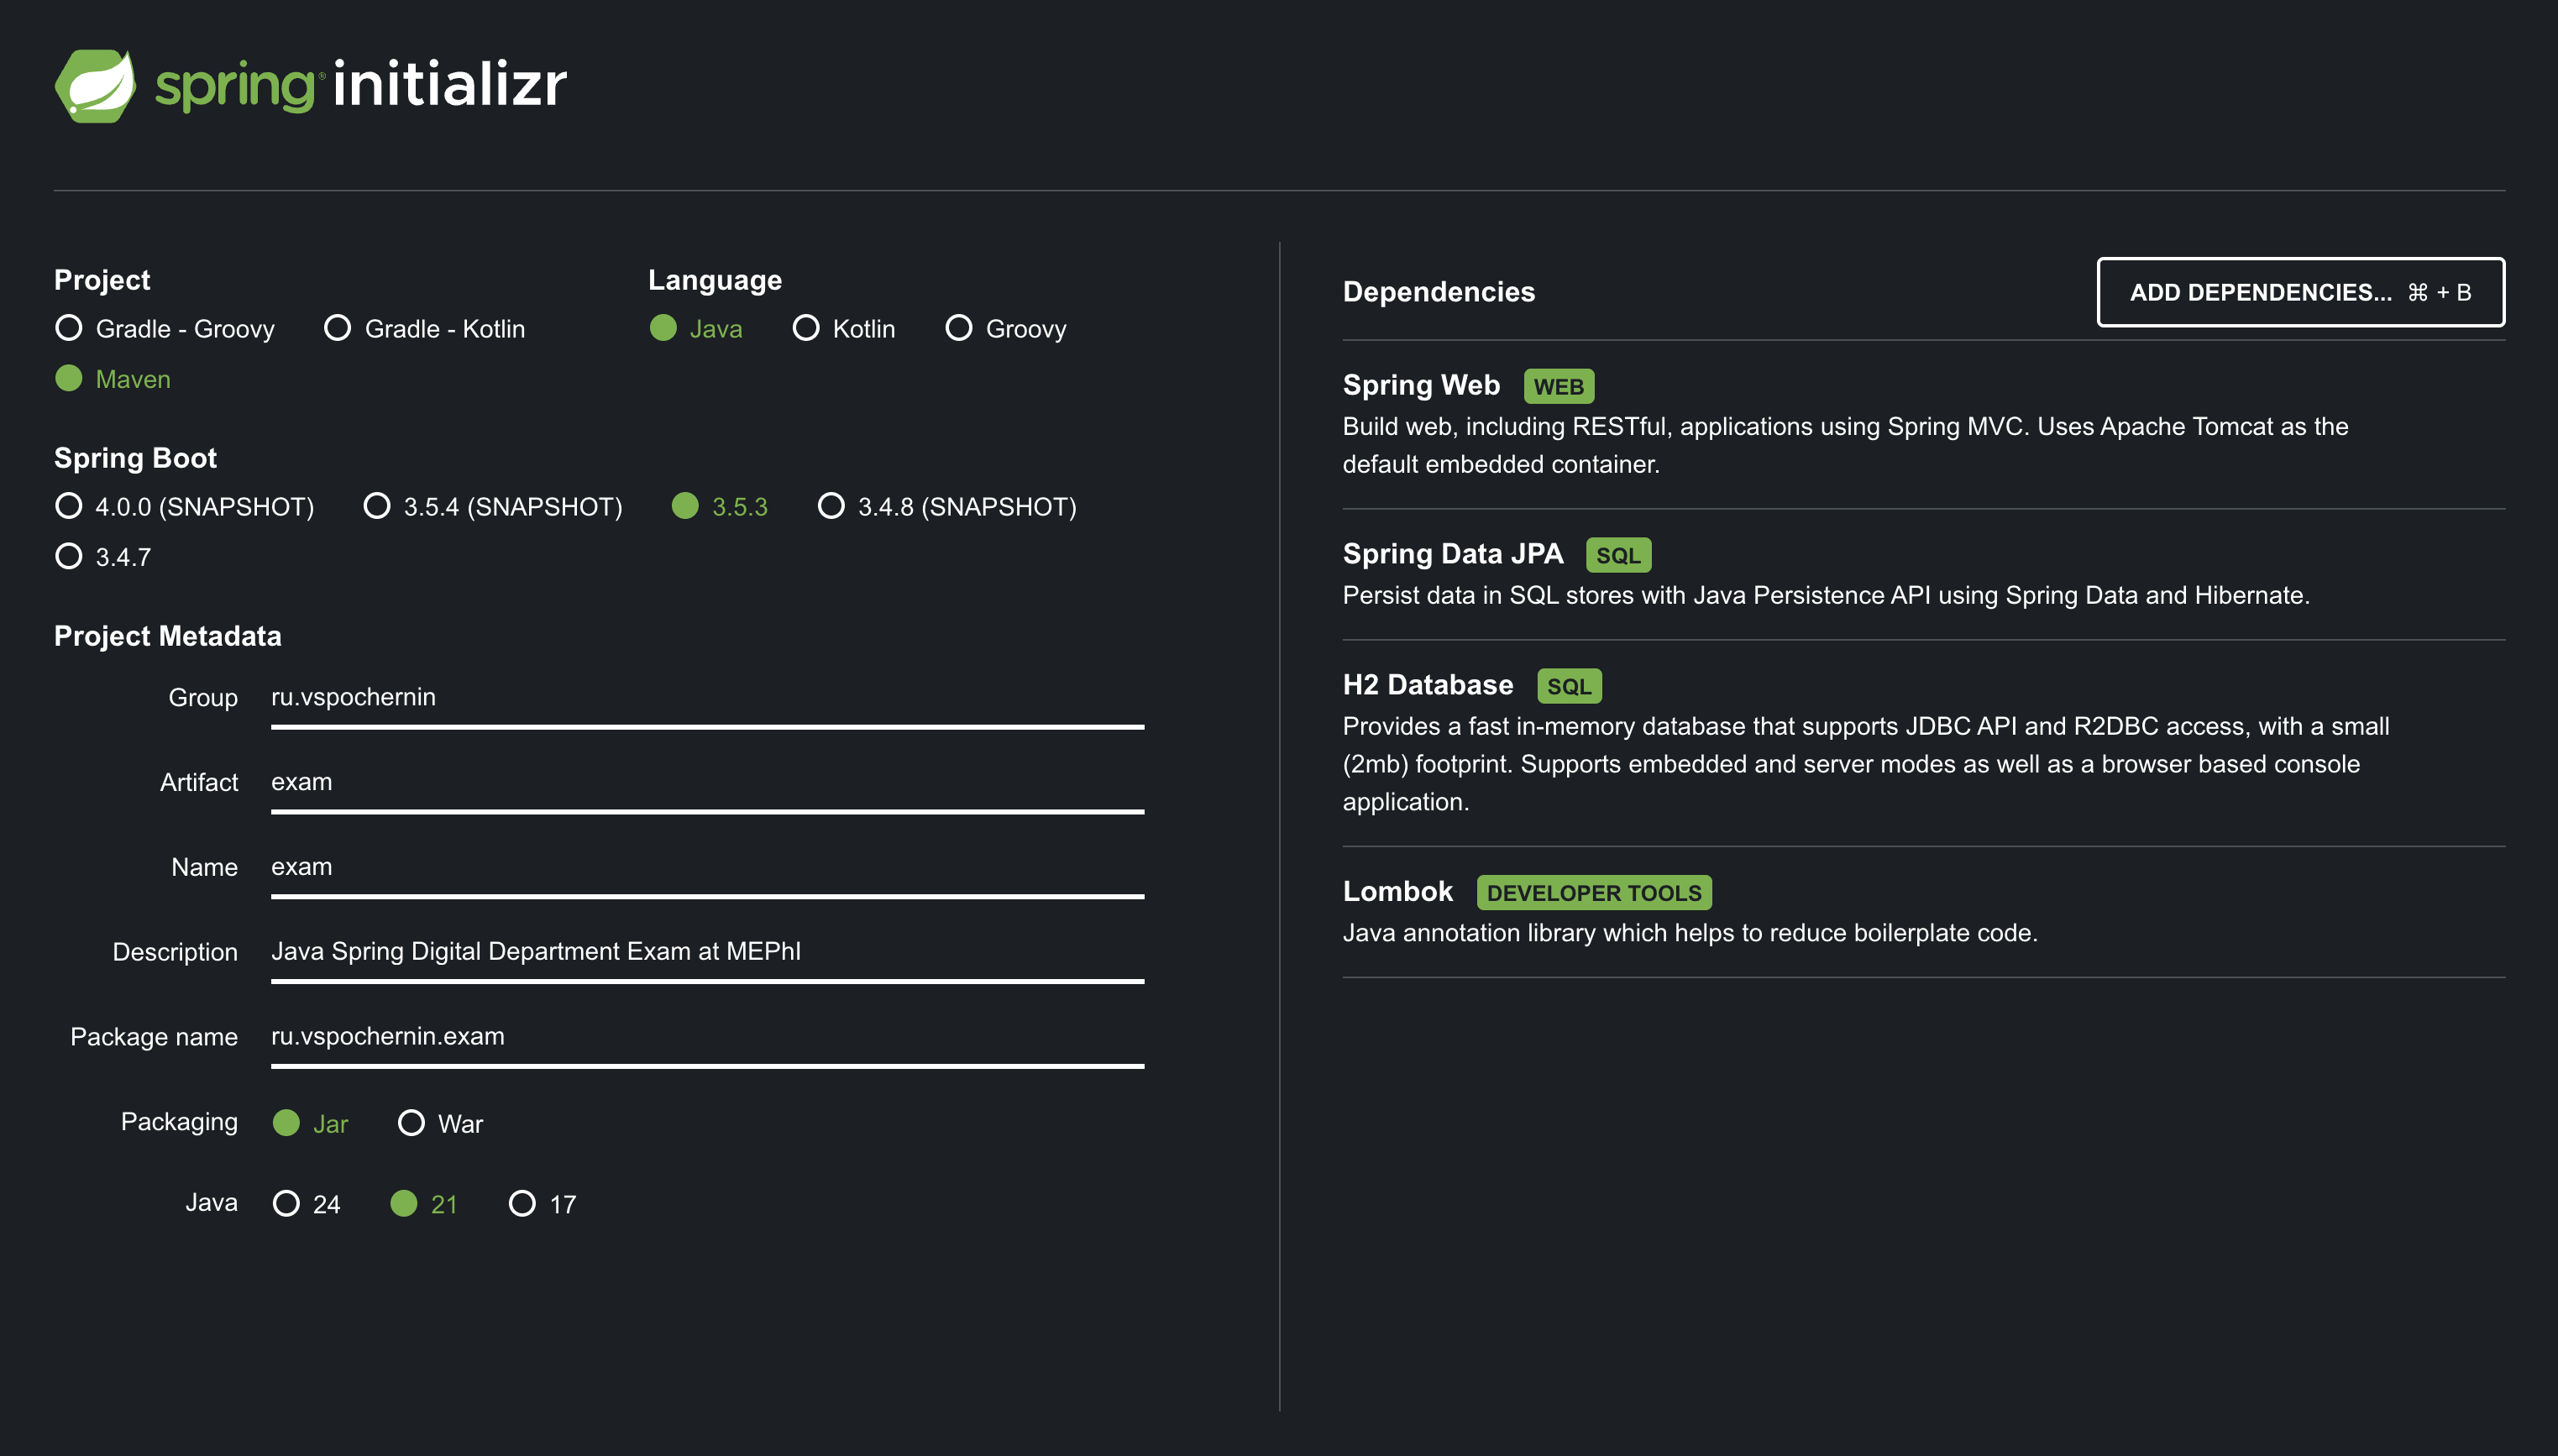
\includegraphics[width=17cm]{resources/1.png}
	\caption{Инициализация проекта}
\end{figure}

Мы будем использовать Java версии 21, сборщик Maven, а также актуальную на момент написания отчета версию Spring Boot - 3.5.3.


Из зависимостей были выбраны:

\begin{itemize}
	\item Spring Web - для создания сервера, который сможет отвечать на HTTP запросы.
	\item Spring Data JPA - для взаимодействия с нашей H2 базой данных с помощью объектно-реляционного отображения.
	\item H2 Database - драйвер для работы H2 базы данных.
	\item Lombok - вспомогательный инструмент для уменьшения количества boilerplate кода.
\end{itemize}

\subsection{Написание кода}

\subsubsection{Пакет model}

Для начала реализуем классы-модели.

Создадим enum \texttt{Country}, задающий 5 стран:

\normalsize
\inputminted[frame=single]{Java}{../src/main/java/ru/vspochernin/exam/model/Country.java}
\large

А также класс пользователя, который будет связан с таблицей \texttt{users} базы данных:

\normalsize
\inputminted[frame=single]{Java}{../src/main/java/ru/vspochernin/exam/model/User.java}
\large

Важными моментами здесь является аннотация \texttt{@Table(name = "users")}, задающая название таблицы БД, а также аннотация \texttt{@Enumerated(EnumType.STRING)}, объясняющая, что enum нужно обрабатывать как строку (без нее в базу записывались бы порядковые номера). \texttt{@GeneratedValue(strategy = GenerationType.IDENTITY)} над полем \texttt{id} делегирует установку ID на уровень базы данных, нам не нужно будет задумываться об этом (например, при добавлении пользователей мы будем использовать конструктор без поля \texttt{id}, но база данных сама проставит это поле в модель).

\subsubsection{Пакет repository}

Далее реализуем класс-репозиторий для пользователя:

\normalsize
\inputminted[frame=single]{Java}{../src/main/java/ru/vspochernin/exam/repository/UserRepository.java}
\large

Здесь мы добавили метод \texttt{findByAgeGreaterThanEqualOrderByFirstNameAsc} для того, чтобы использовать его в эндпоинте \texttt{additional-info}.

Важный момент: хотя в задании сказано использовать соответствующие слоям Spring аннотации, в репозитории совсем не обязательно ставить аннотацию \texttt{@Repository}, в случае, если это \texttt {JPA Repository} (\url{https://stackoverflow.com/questions/44069367/repository-not-necessary-when-implementing-jparepository}).

\subsubsection{Пакет service}

Создадим класс-сервис для нашей программы:

\normalsize
\inputminted[frame=single]{Java}{../src/main/java/ru/vspochernin/exam/service/UserService.java}
\large

Класс использует созданный ранее репозиторий, и в нем реализованы методы для получения всех пользователей, добавления нового пользователя, а также для получения списках всех пользователей, возраст которых больше либо равен заданному, отсортированный по имени (\texttt{firstName}) в алфавитном порядке.

\subsubsection{Пакет controller}

Наконец, реализуем контроллер для обработки входящих запросов:

\normalsize
\inputminted[frame=single]{Java}{../src/main/java/ru/vspochernin/exam/controller/UserController.java}
\large

Для соответствия условиям задачи здесь задается базовый путь с помощью аннотации \texttt{@RequestMapping("/user-api/v1")}. А в случае создания пользователя также возвращается статус 201 CREATED (вместо стандартного 200 OK) с помощью аннотации \texttt{@ResponseStatus(HttpStatus.CREATED)}.

\subsubsection{Наполнение БД}

Для наполнения базы данных при старте приложения был модернизирован созданный при инициализации проекта файл \texttt{ExamApplication}.

\normalsize
\inputminted[frame=single]{Java}{../src/main/java/ru/vspochernin/exam/ExamApplication.java}
\large

В него был добавлен бин \texttt{CommandLineRunner}, который при запуске сохранял в репозиторий (то есть в нашу базу) 5 пользователей.

\subsubsection{Конфигурация}

Для того, чтобы наше приложение работало корректно, нам нужно настроить его в файле \texttt{application.properties}:

\normalsize
\inputminted[frame=single]{properties}{../src/main/resources/application.properties}
\large

В начале файла задается имя приложения. Затем настраивается соединение с БД (адрес, тип драйвера, логин и пароль). Далее мы указываем нужный нам диалект, просим Hibernate самому создавать схему БД, а также устанавливаем отображение всех sql запросов, которые генерирует и исполняет Hibernate в консоли. Последняя строка включает админ-панель для нашей БД, к которой можно будет обратиться по адресу \url{http://localhost:8080/h2-console/}.

\subsection{Работа приложения}

\subsubsection{Запуск}

Включим наше приложение, запустим метод \texttt{main()} класса \texttt{ExamApplication}.

\begin{figure}[H]
	\centering
	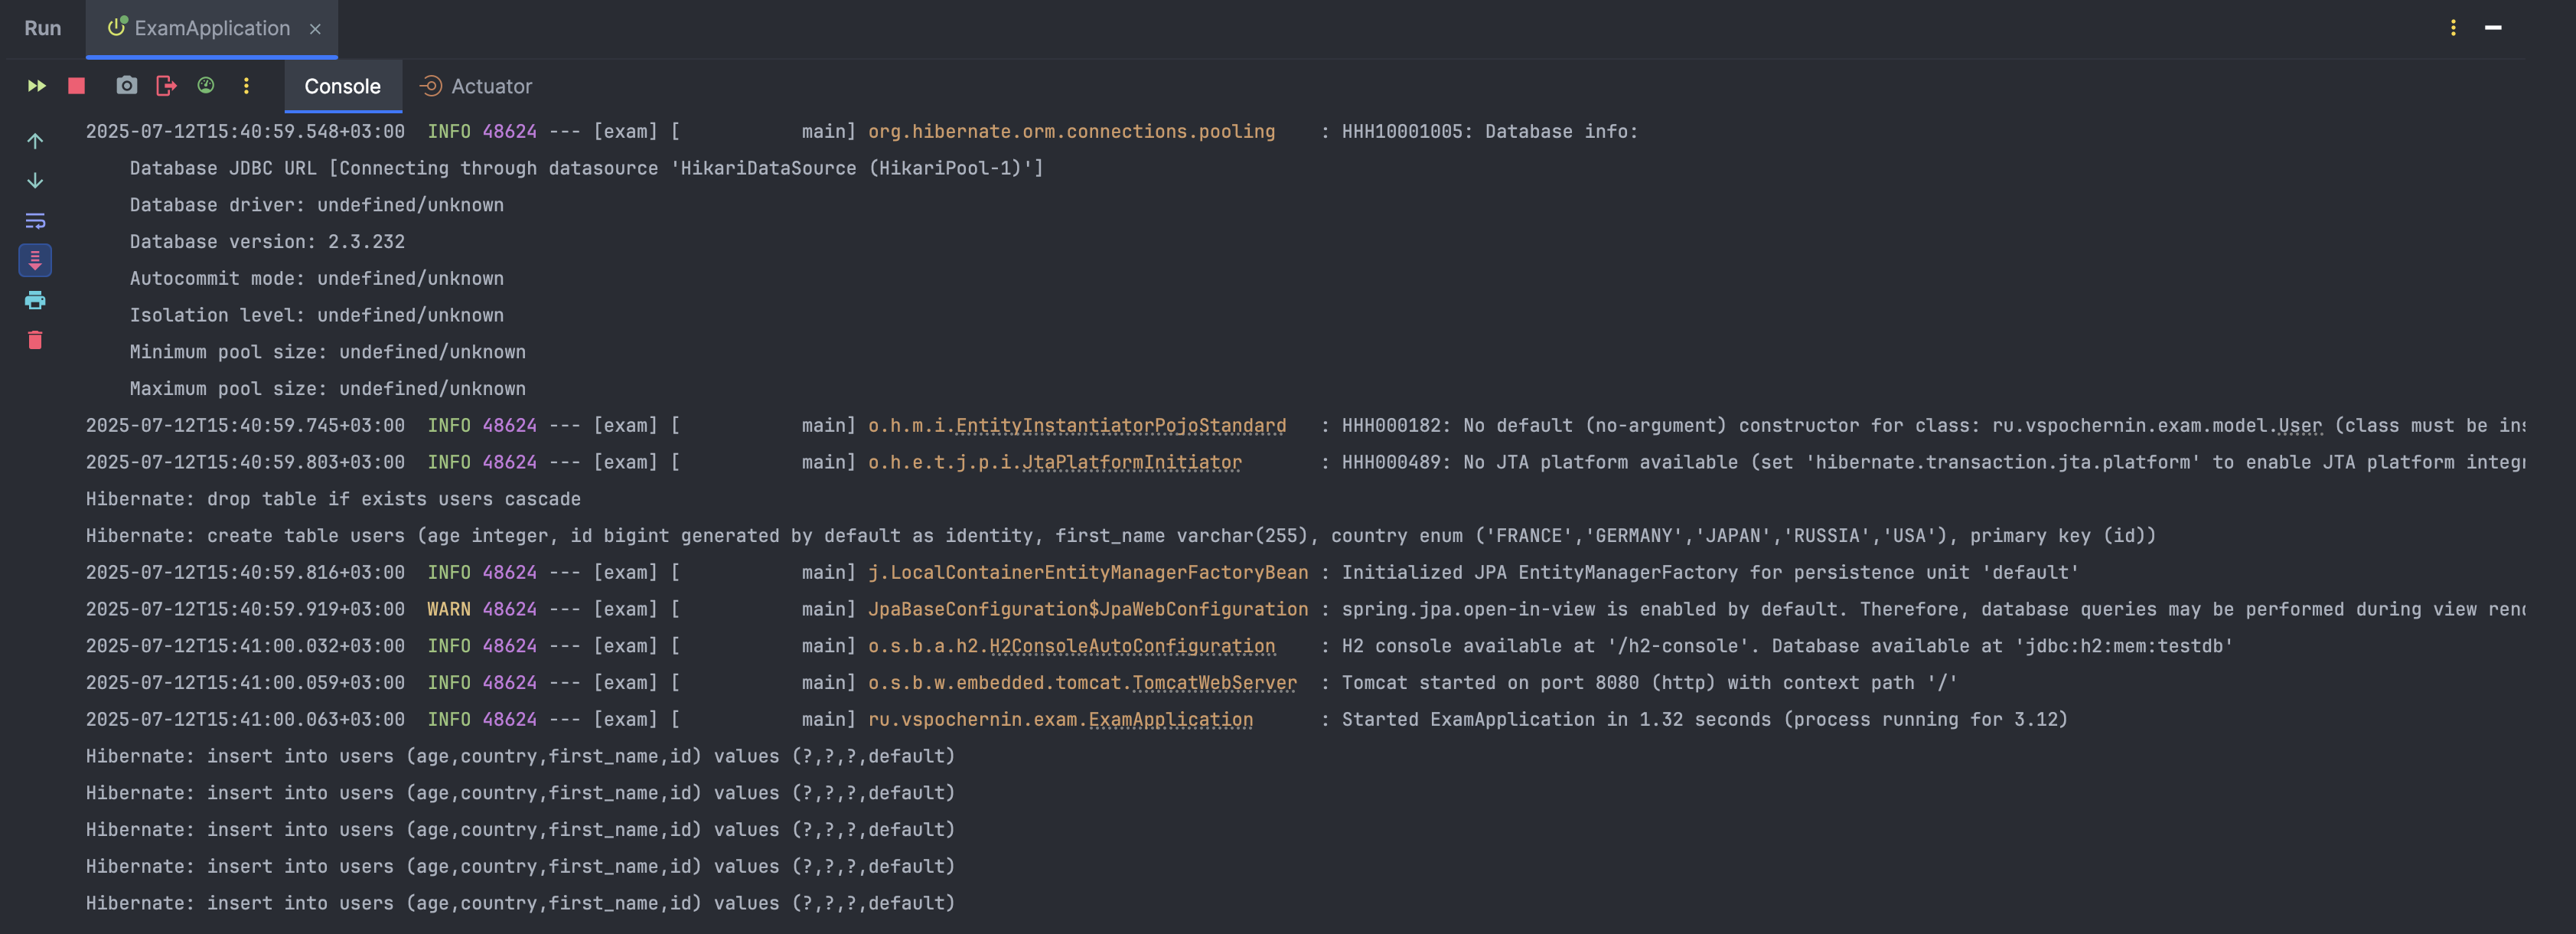
\includegraphics[width=17cm]{resources/2.png}
	\caption{Запуск приложения}
\end{figure}

Из логов в консоли можно увидеть, что у нас успешно инициализировалась база данных, создалась схема БД, а также было добавлено 5 пользователей.

Чтобы убедиться в этом, зайдем в админ-панель базы данных по адресу \url{http://localhost:8080/h2-console/}:

\begin{figure}[H]
	\centering
	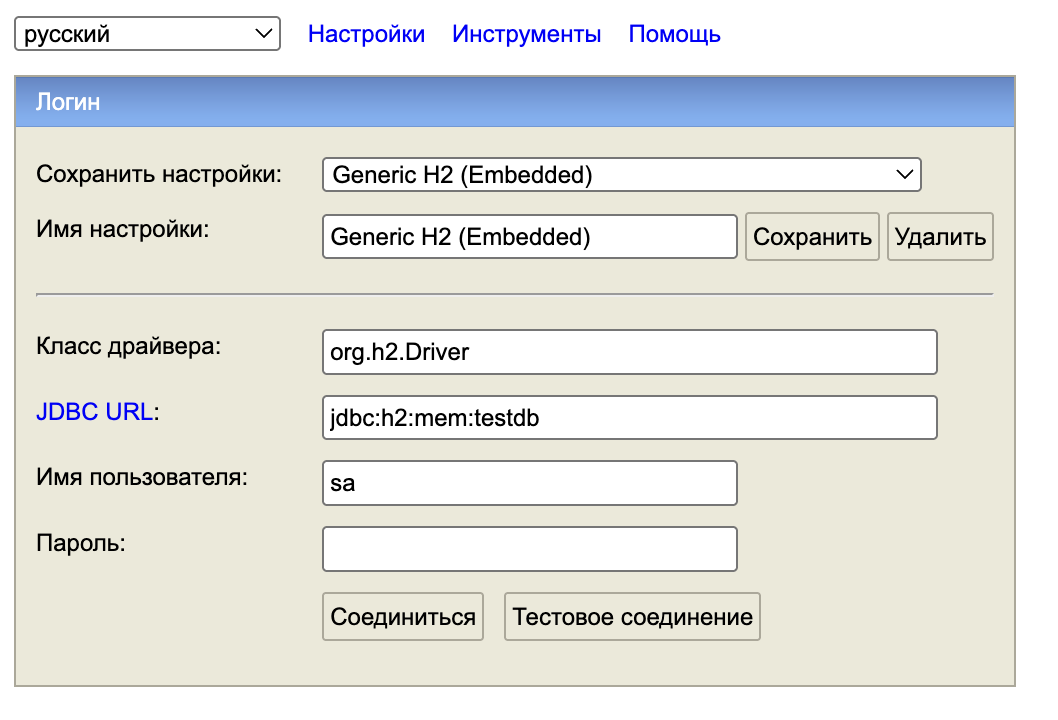
\includegraphics[width=17cm]{resources/3.png}
	\caption{Вход в админ-панель}
\end{figure}

И выполним поиск по всем пользователям:

\begin{figure}[H]
	\centering
	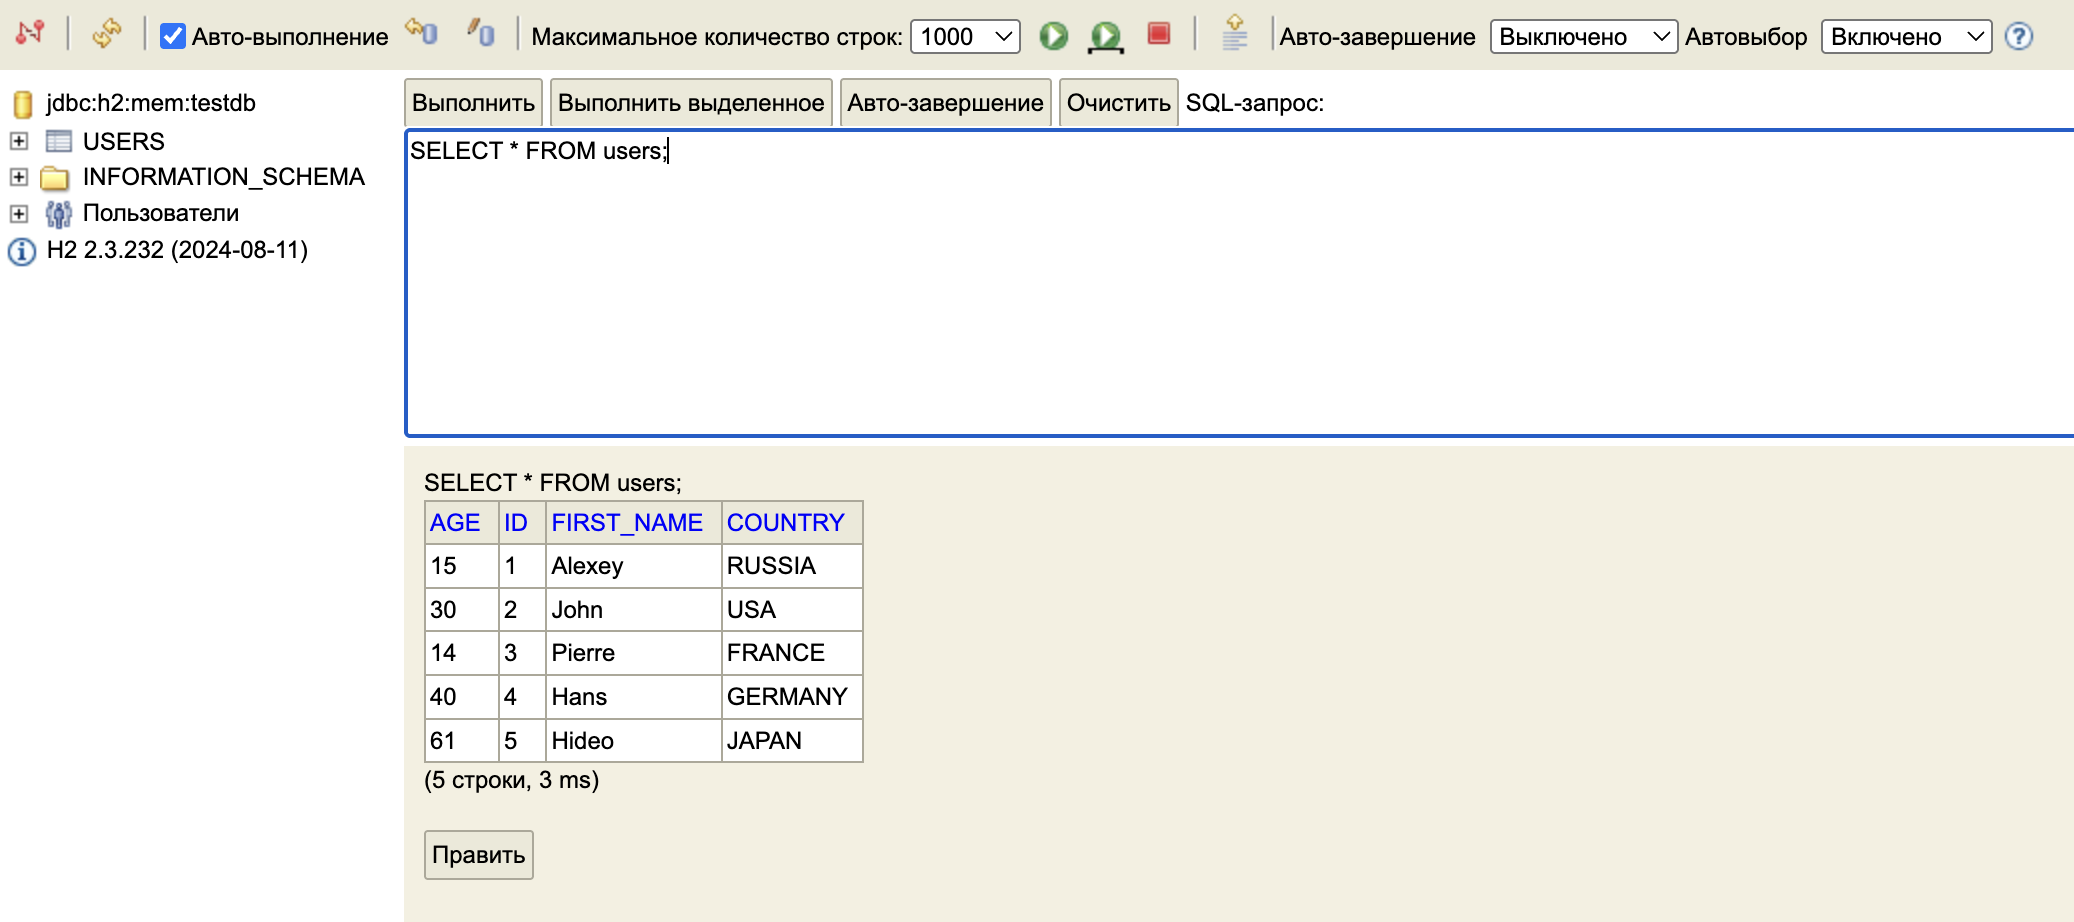
\includegraphics[width=17cm]{resources/4.png}
	\caption{Поиск по всем пользователям}
\end{figure}

Как можно заметить, в базу действительно добавились те пользователи, которых мы указывали в коде.

\subsubsection{Проверка запросов}

Проверим работу наших запросов. Для этого будем использовать Postman.

Выполним первый запрос и получим список всех пользователей:

\begin{figure}[H]
	\centering
	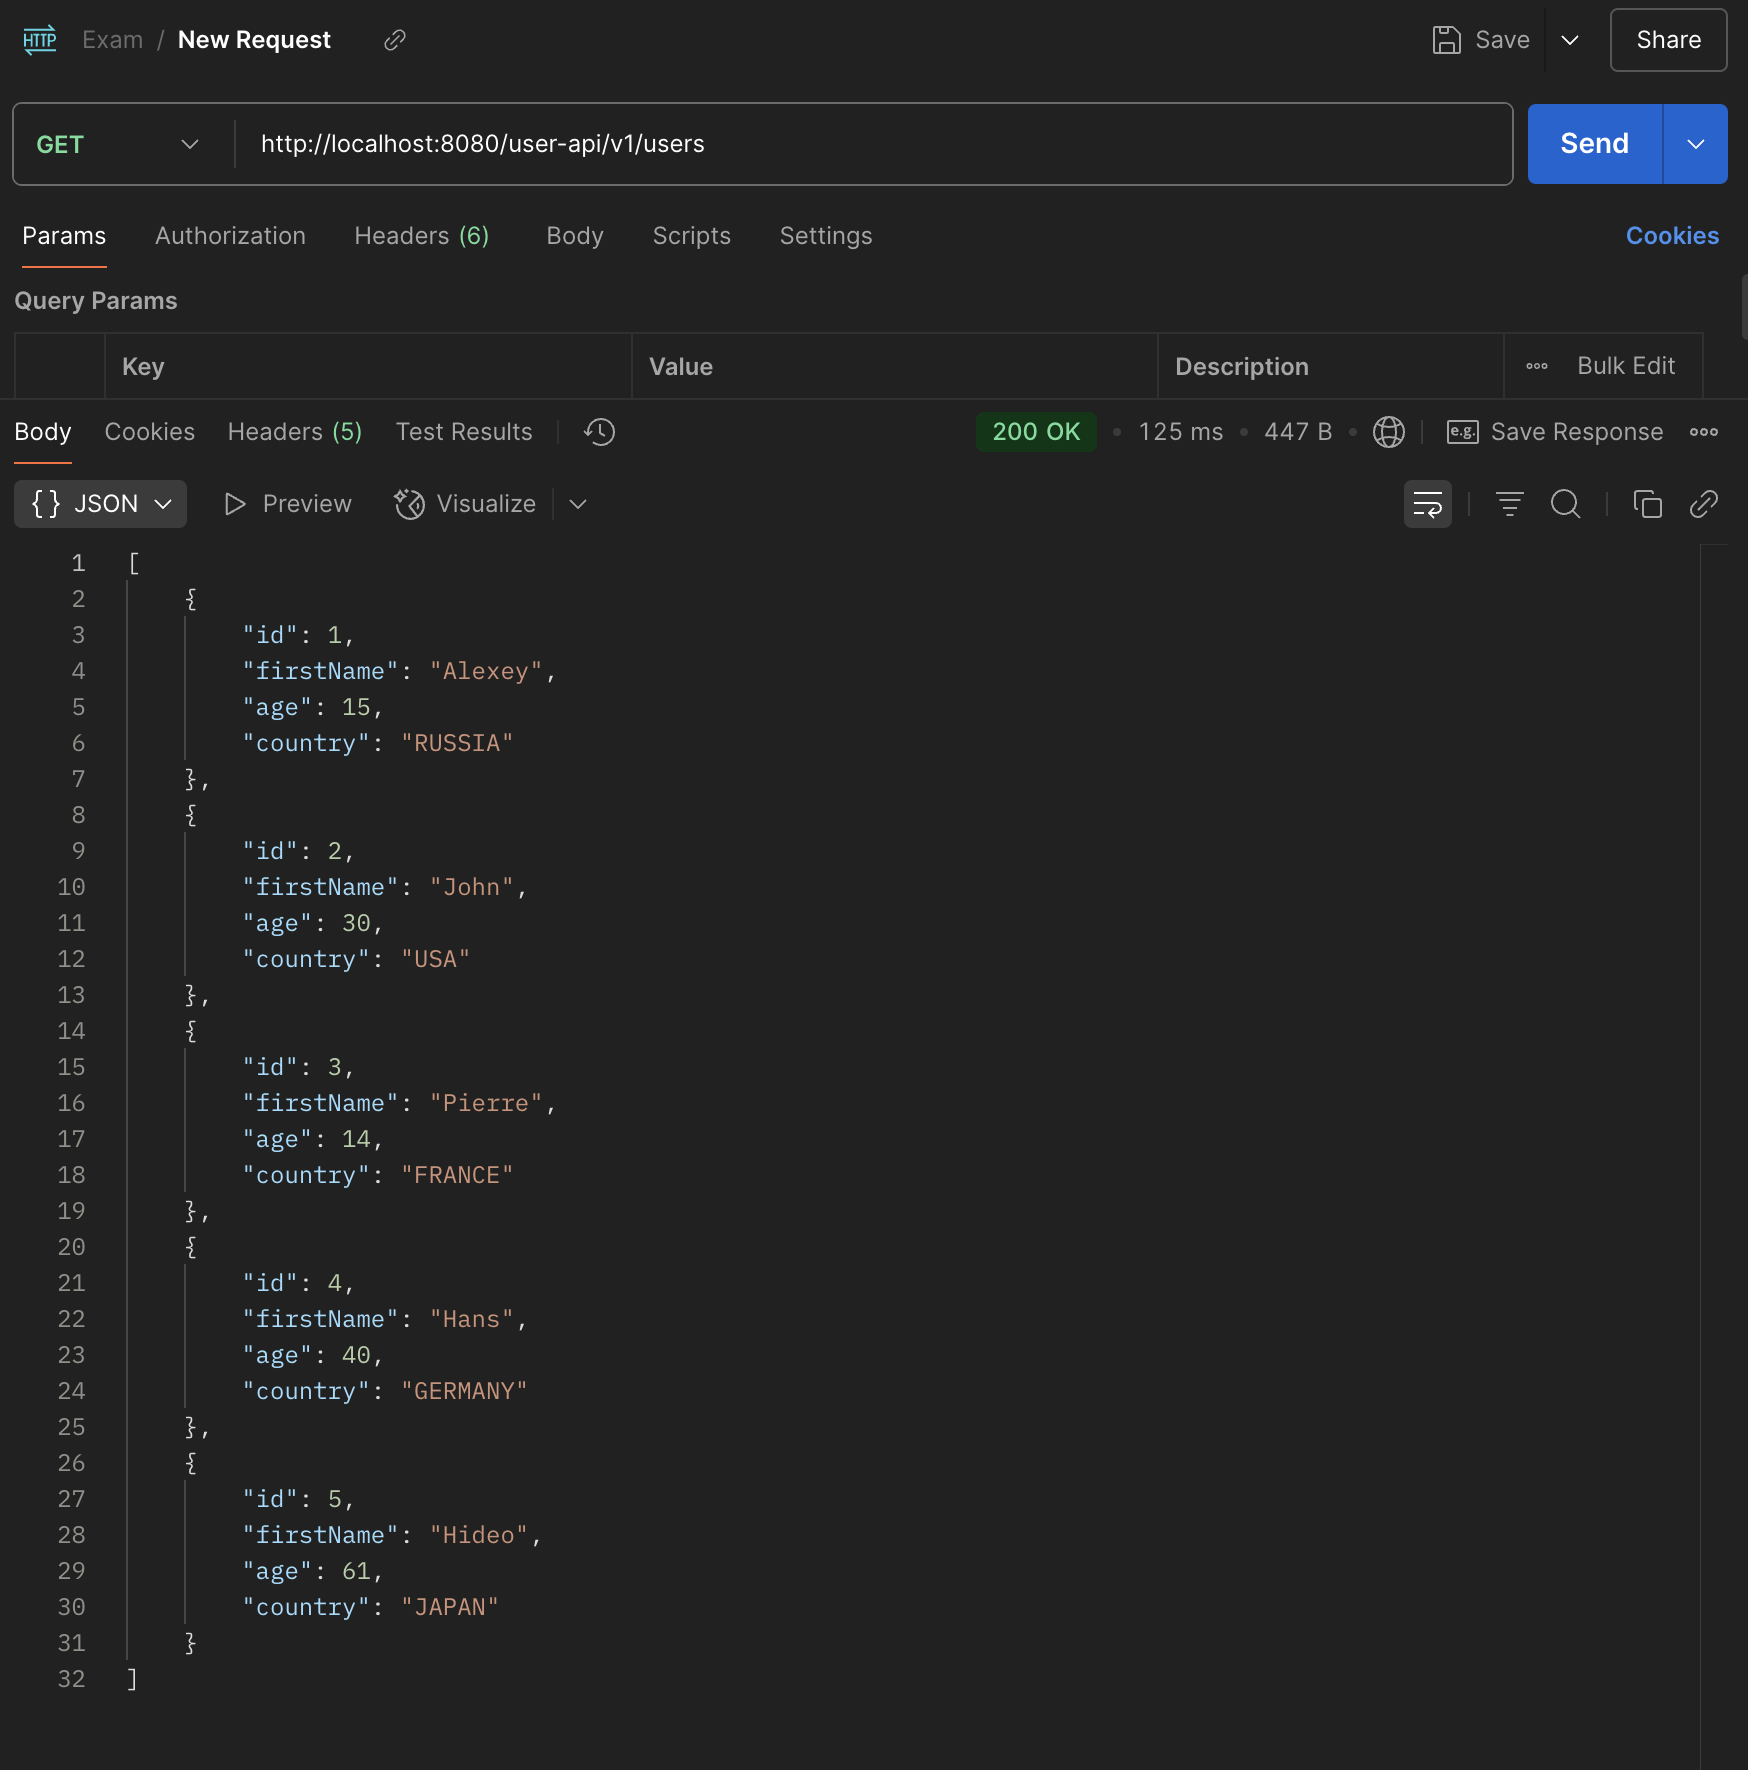
\includegraphics[width=15cm]{resources/5.png}
	\caption{Получение списка всех пользователей}
\end{figure}

Далее выполним два запроса, чтобы добавить двух новых пользователей:

\begin{figure}[H]
	\centering
	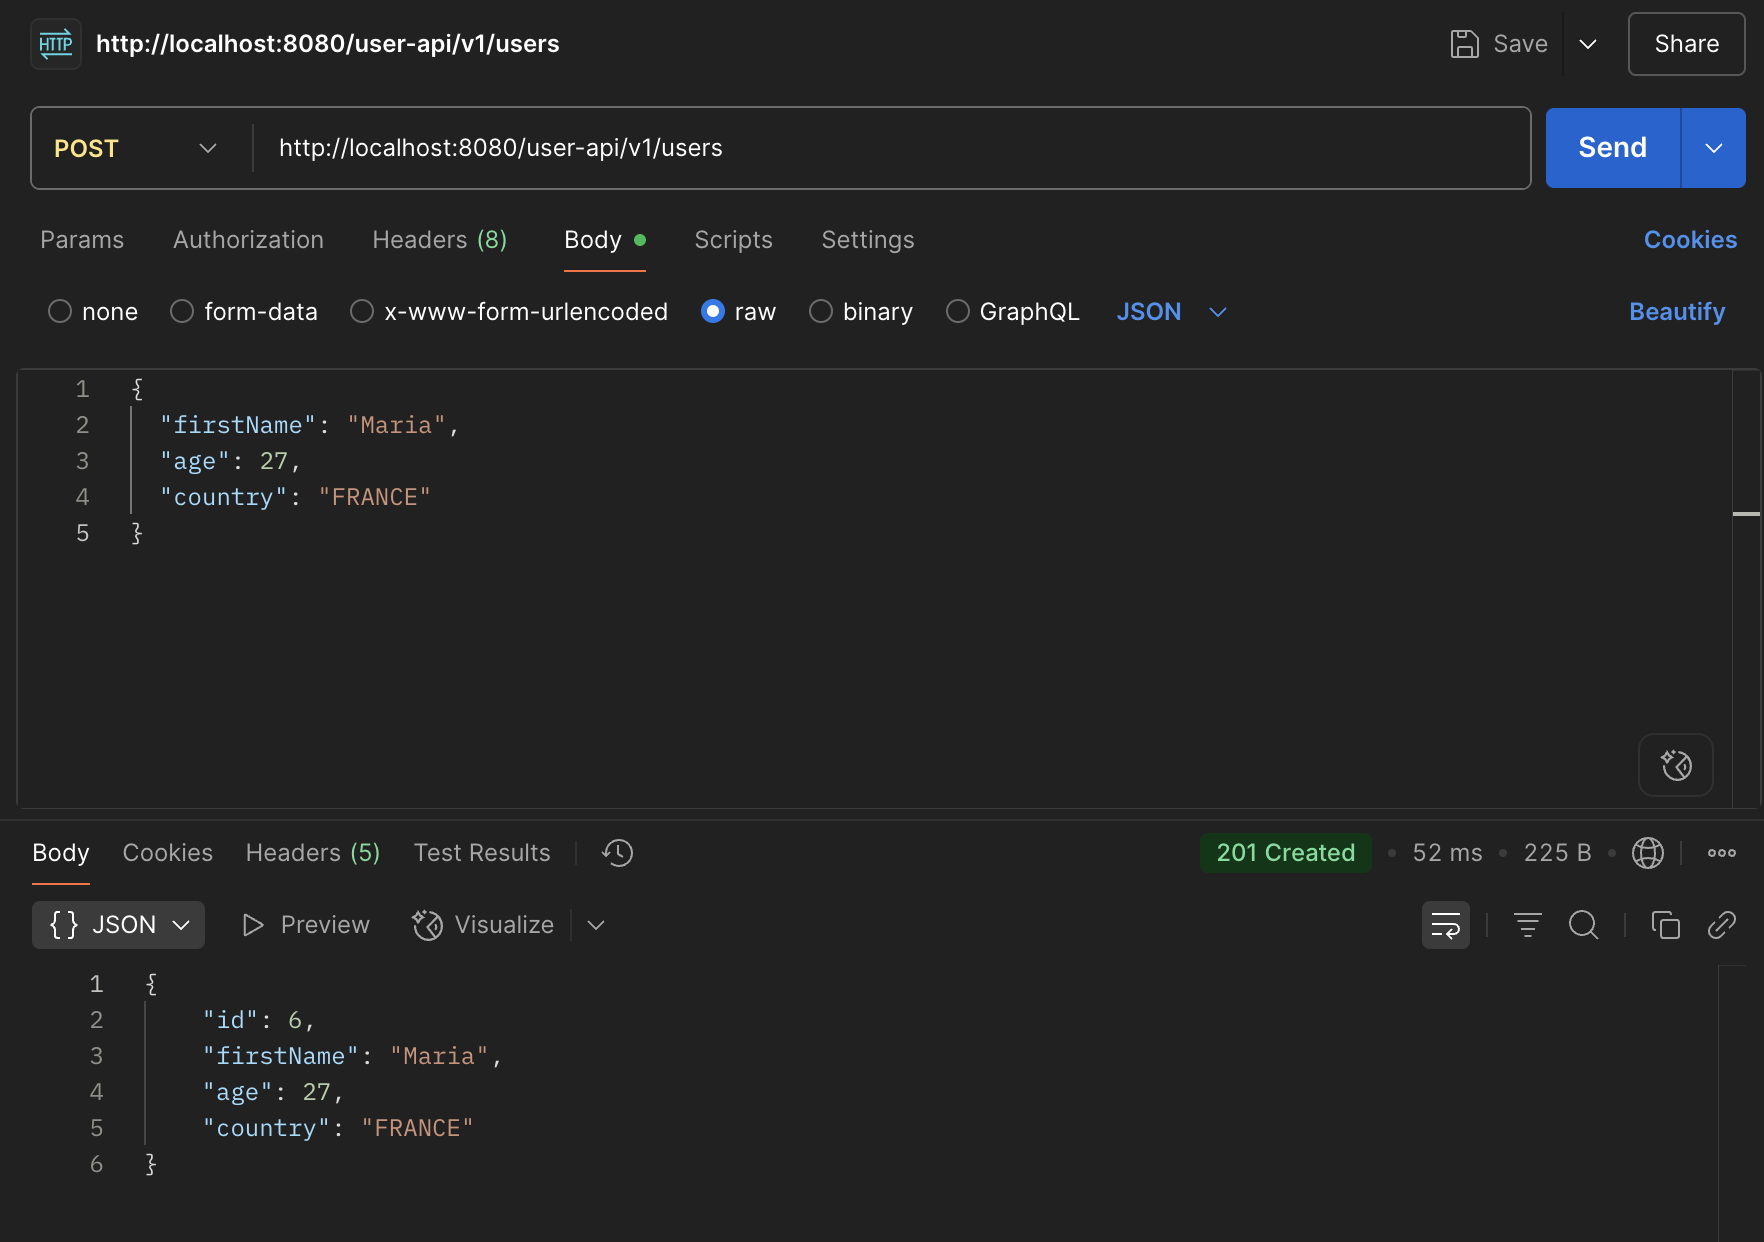
\includegraphics[width=15cm]{resources/6.png}
	\caption{Добавление пользователя Marina}
\end{figure}

\begin{figure}[H]
	\centering
	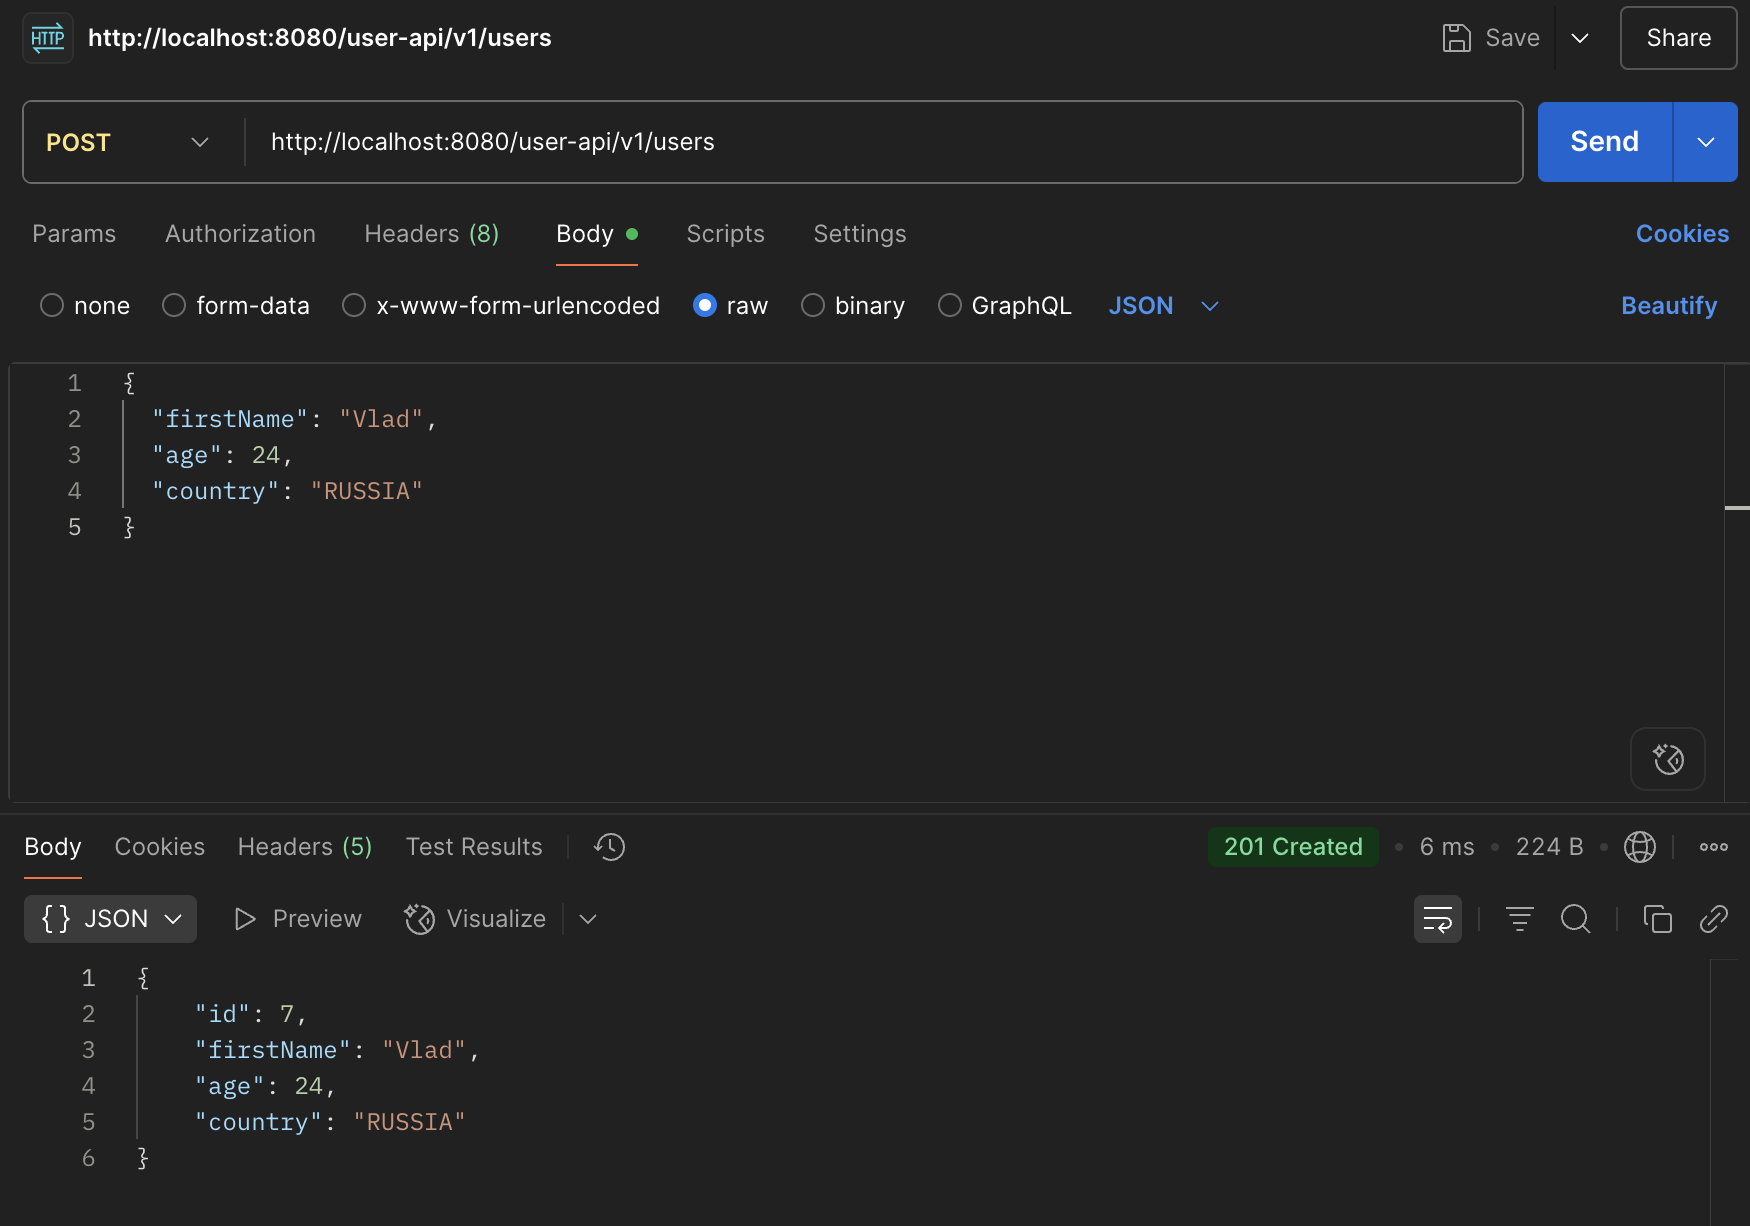
\includegraphics[width=15cm]{resources/7.png}
	\caption{Добавление пользователя Vlad}
\end{figure}

Снова запросив всех пользователей, увидим, что новые также появились в списке:

\begin{figure}[H]
	\centering
	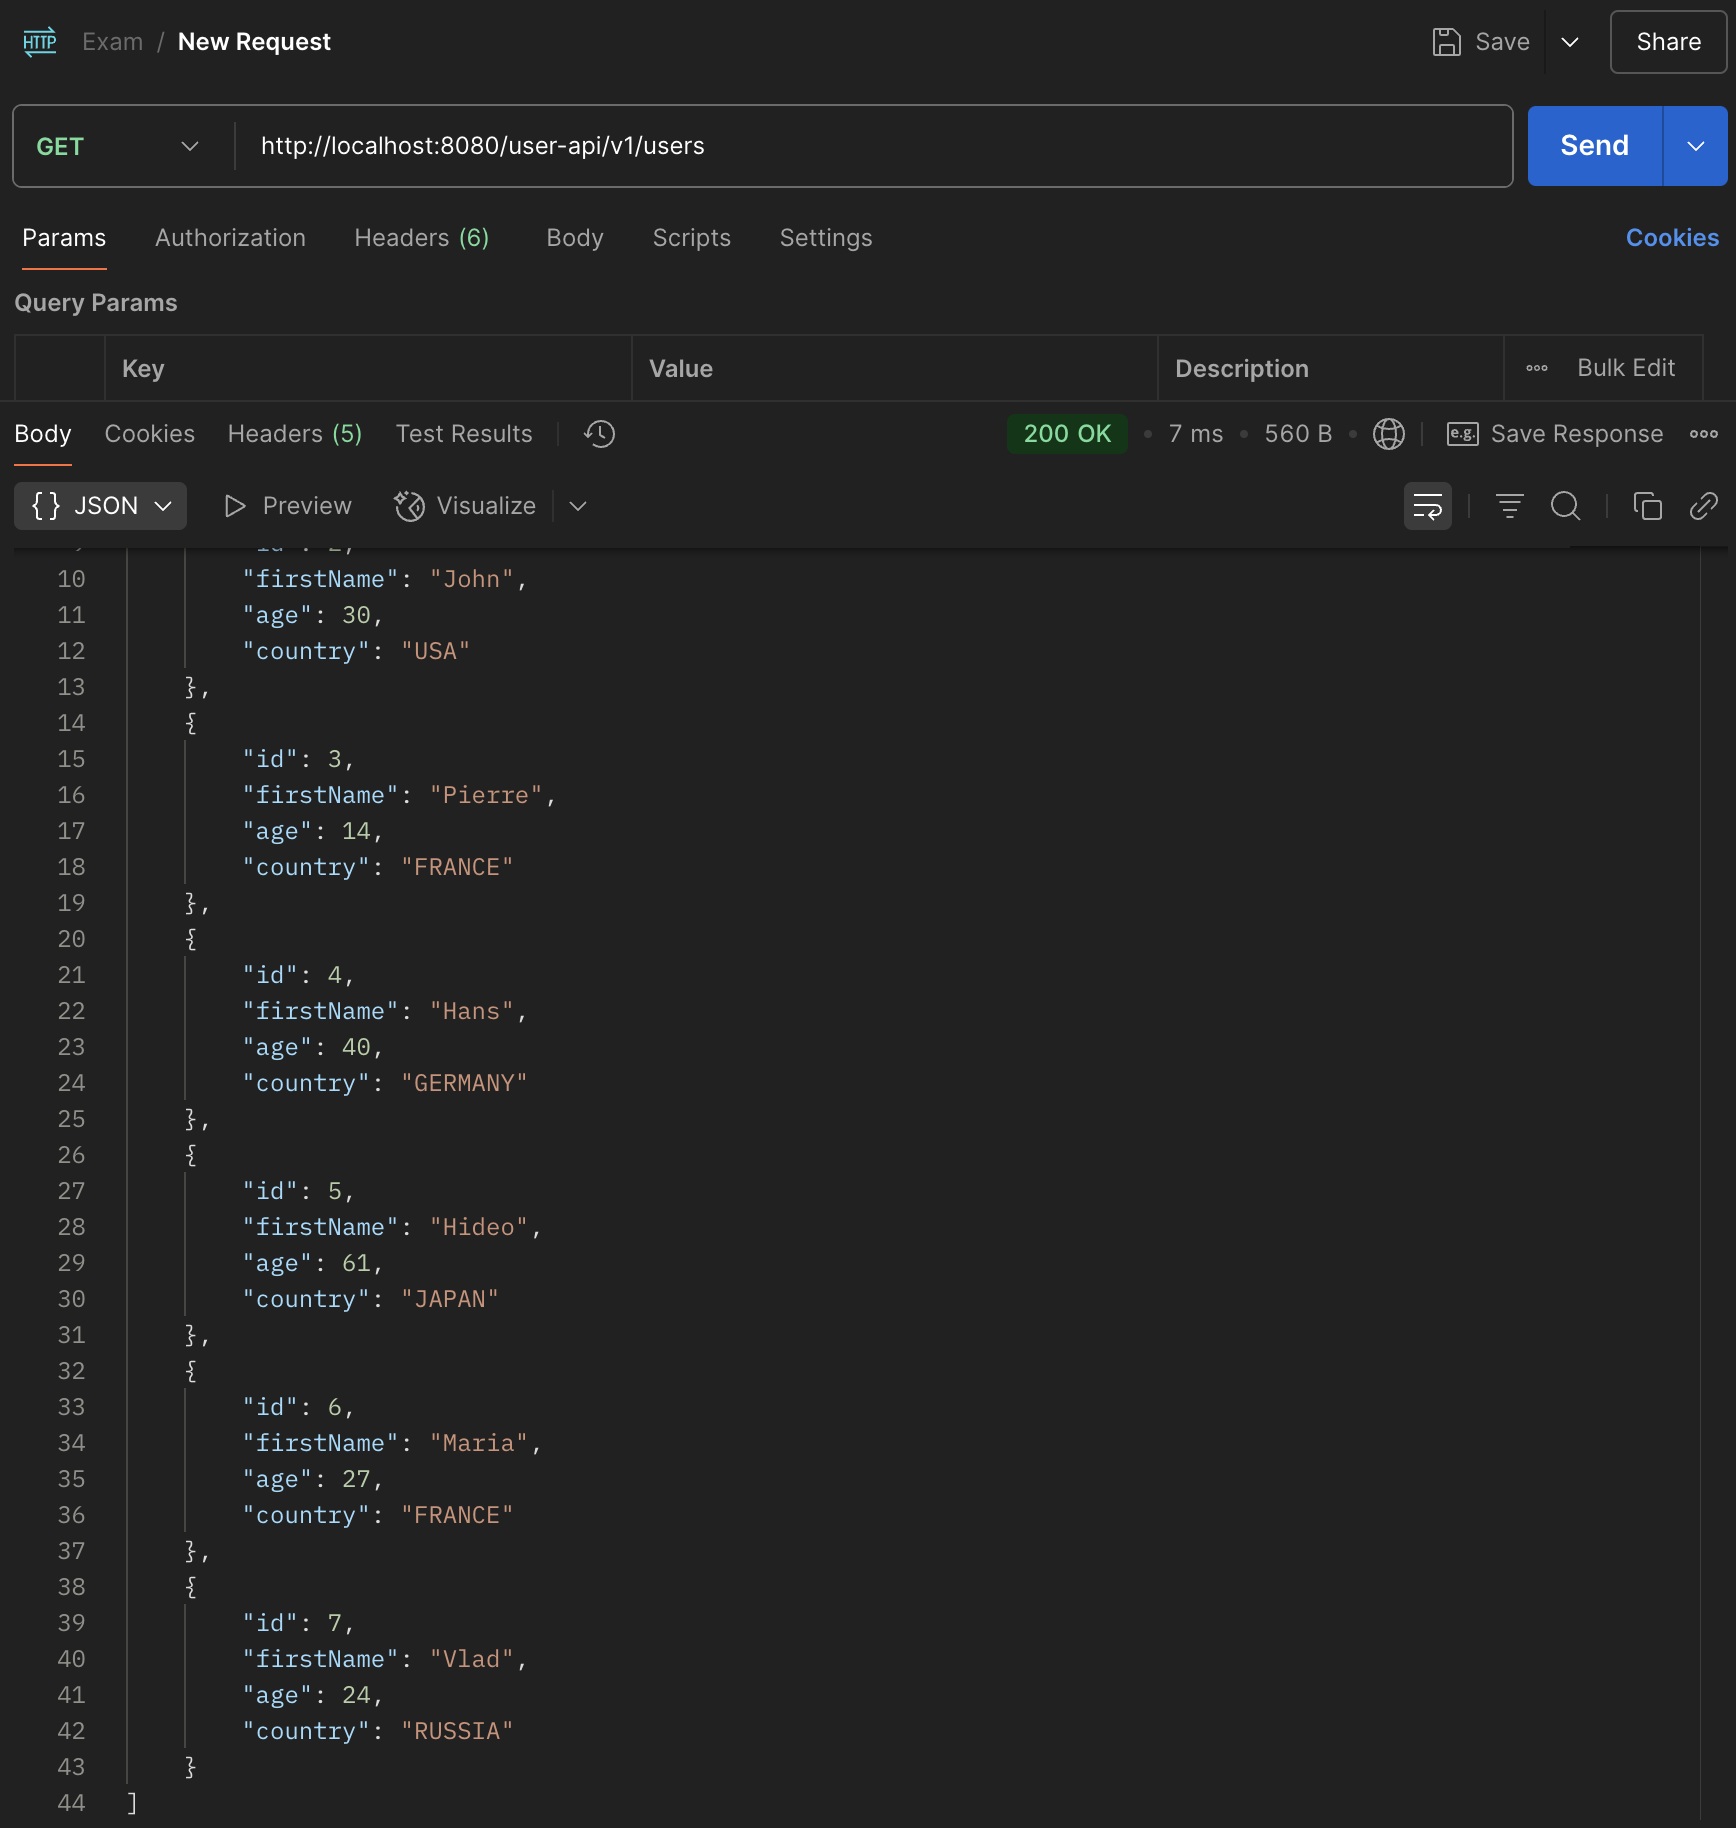
\includegraphics[width=15cm]{resources/8.png}
	\caption{Получение списка всех пользователей после добавления новых}
\end{figure}

Наконец, протестируем эндпоинт \texttt{additional-info}.

Сначала забудем передать ему параметр age:

\begin{figure}[H]
	\centering
	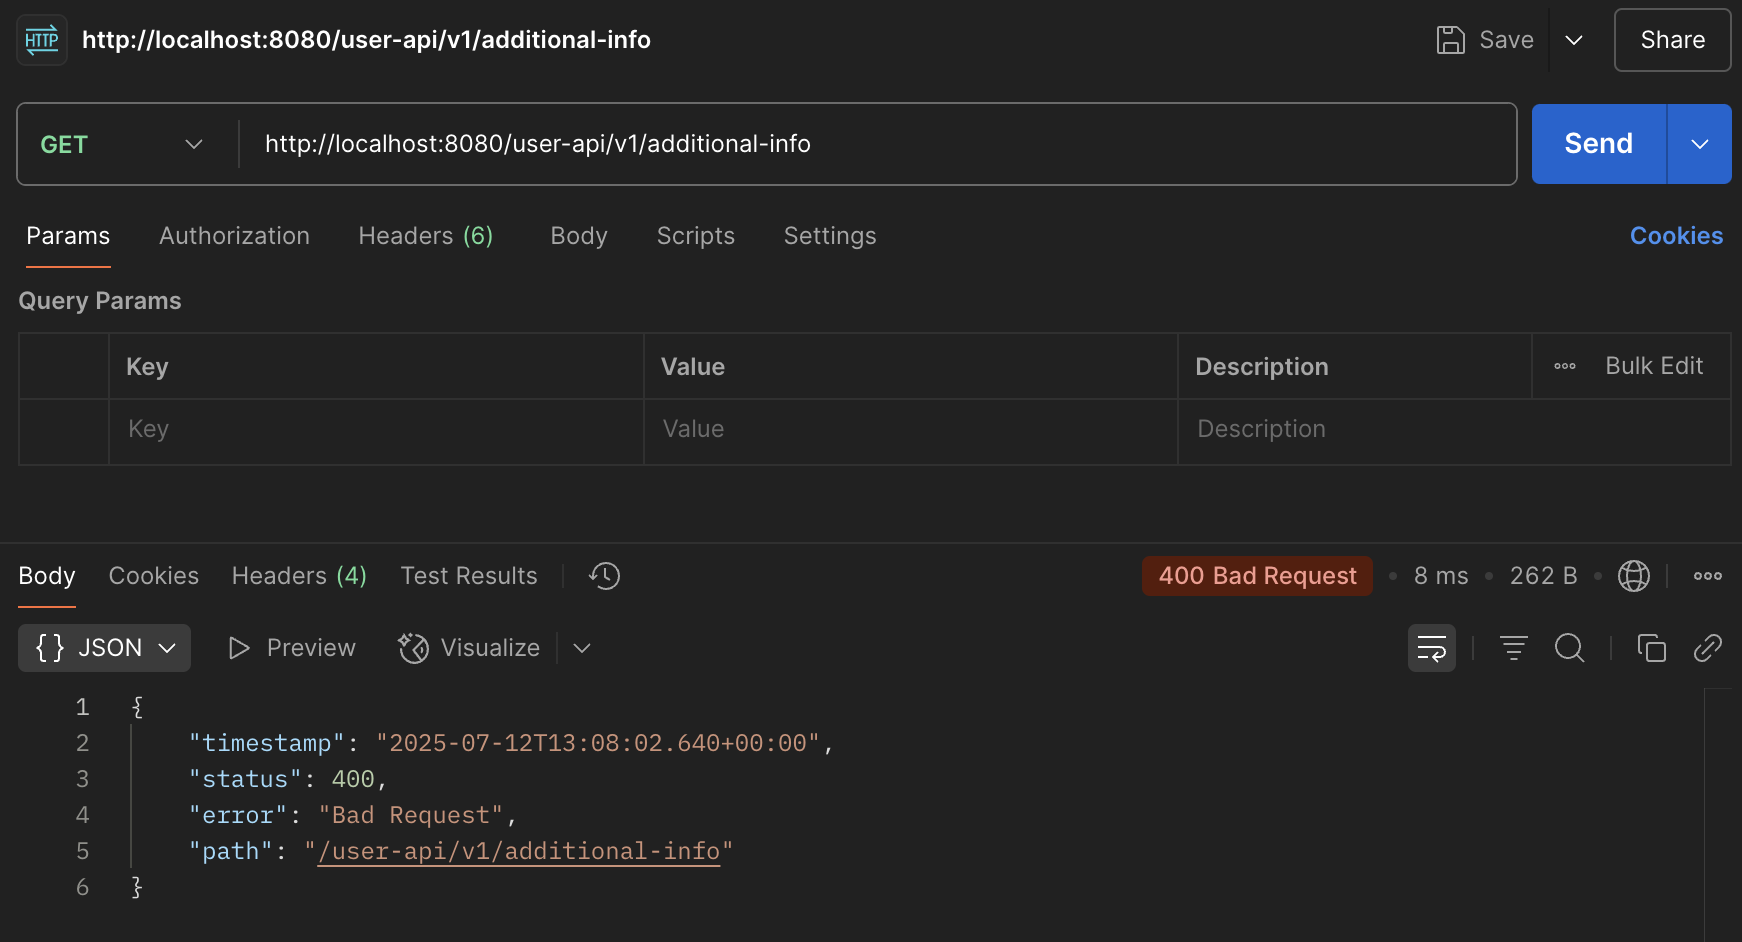
\includegraphics[width=15cm]{resources/9.png}
	\caption{Ошибка на отсутствие параметра age}
\end{figure}

Ту же ошибку получим при попытке передать в age НЕ число:

\begin{figure}[H]
	\centering
	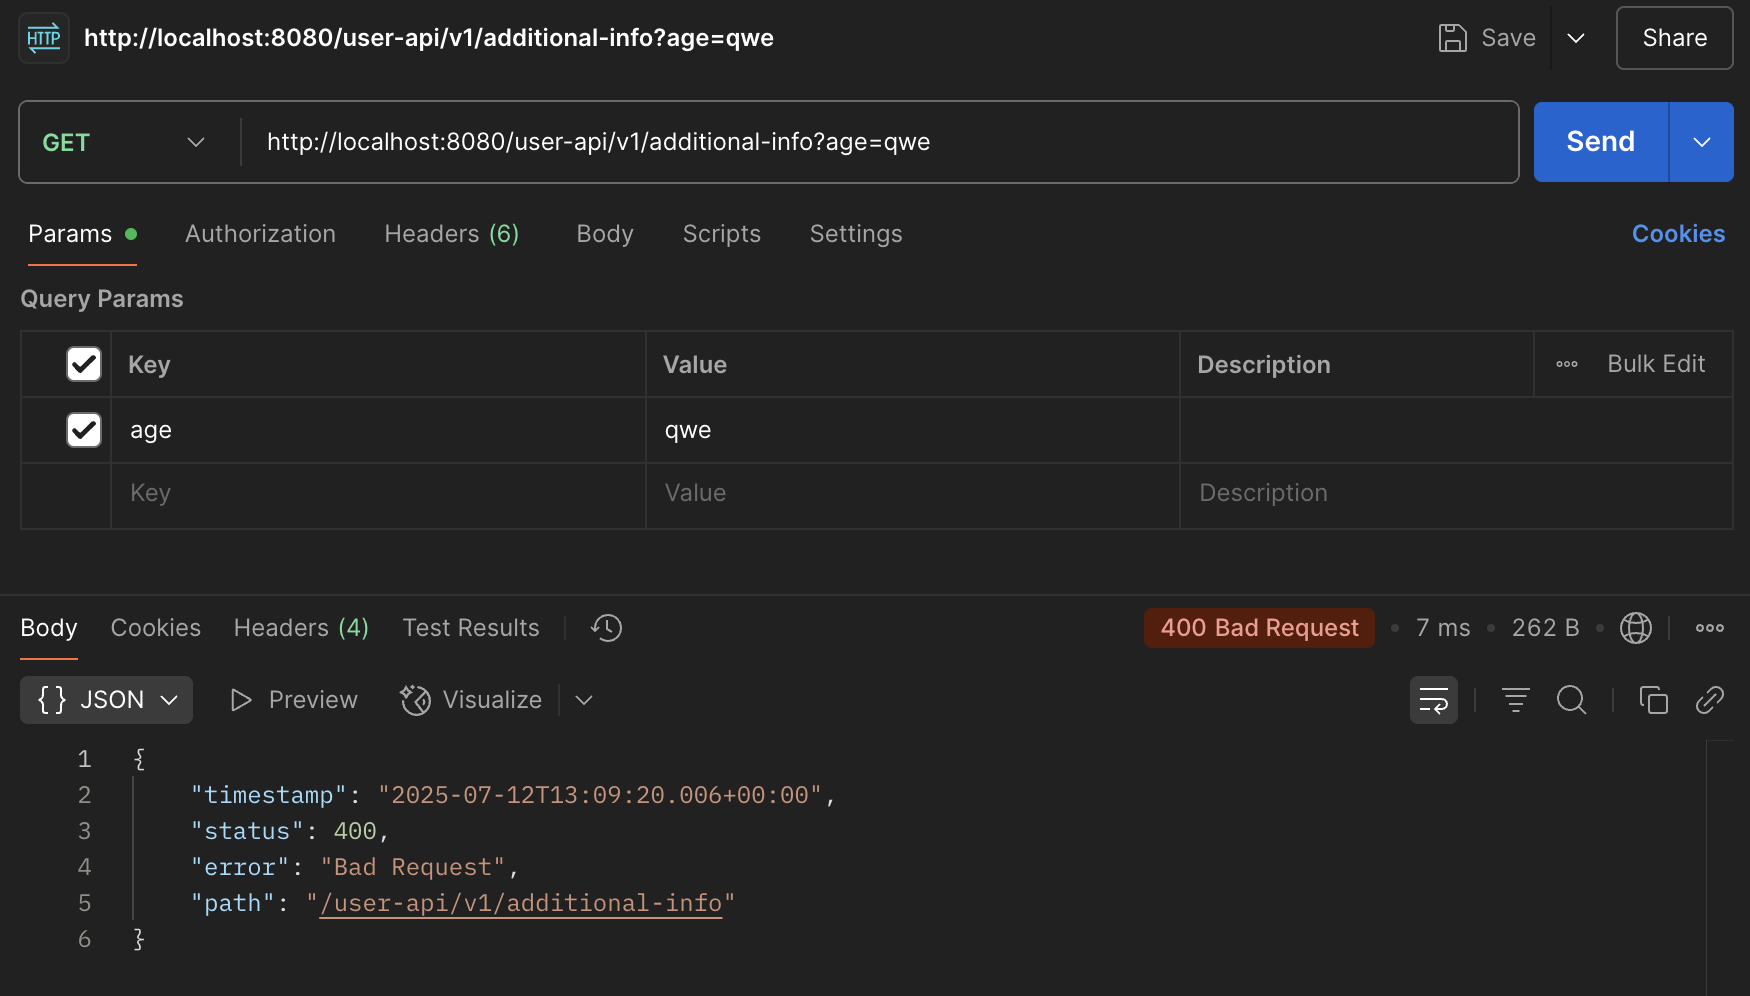
\includegraphics[width=15cm]{resources/10.png}
	\caption{Ошибка на передачу в age НЕ числа}
\end{figure}

Запишем в age отрицательное число:

\begin{figure}[H]
	\centering
	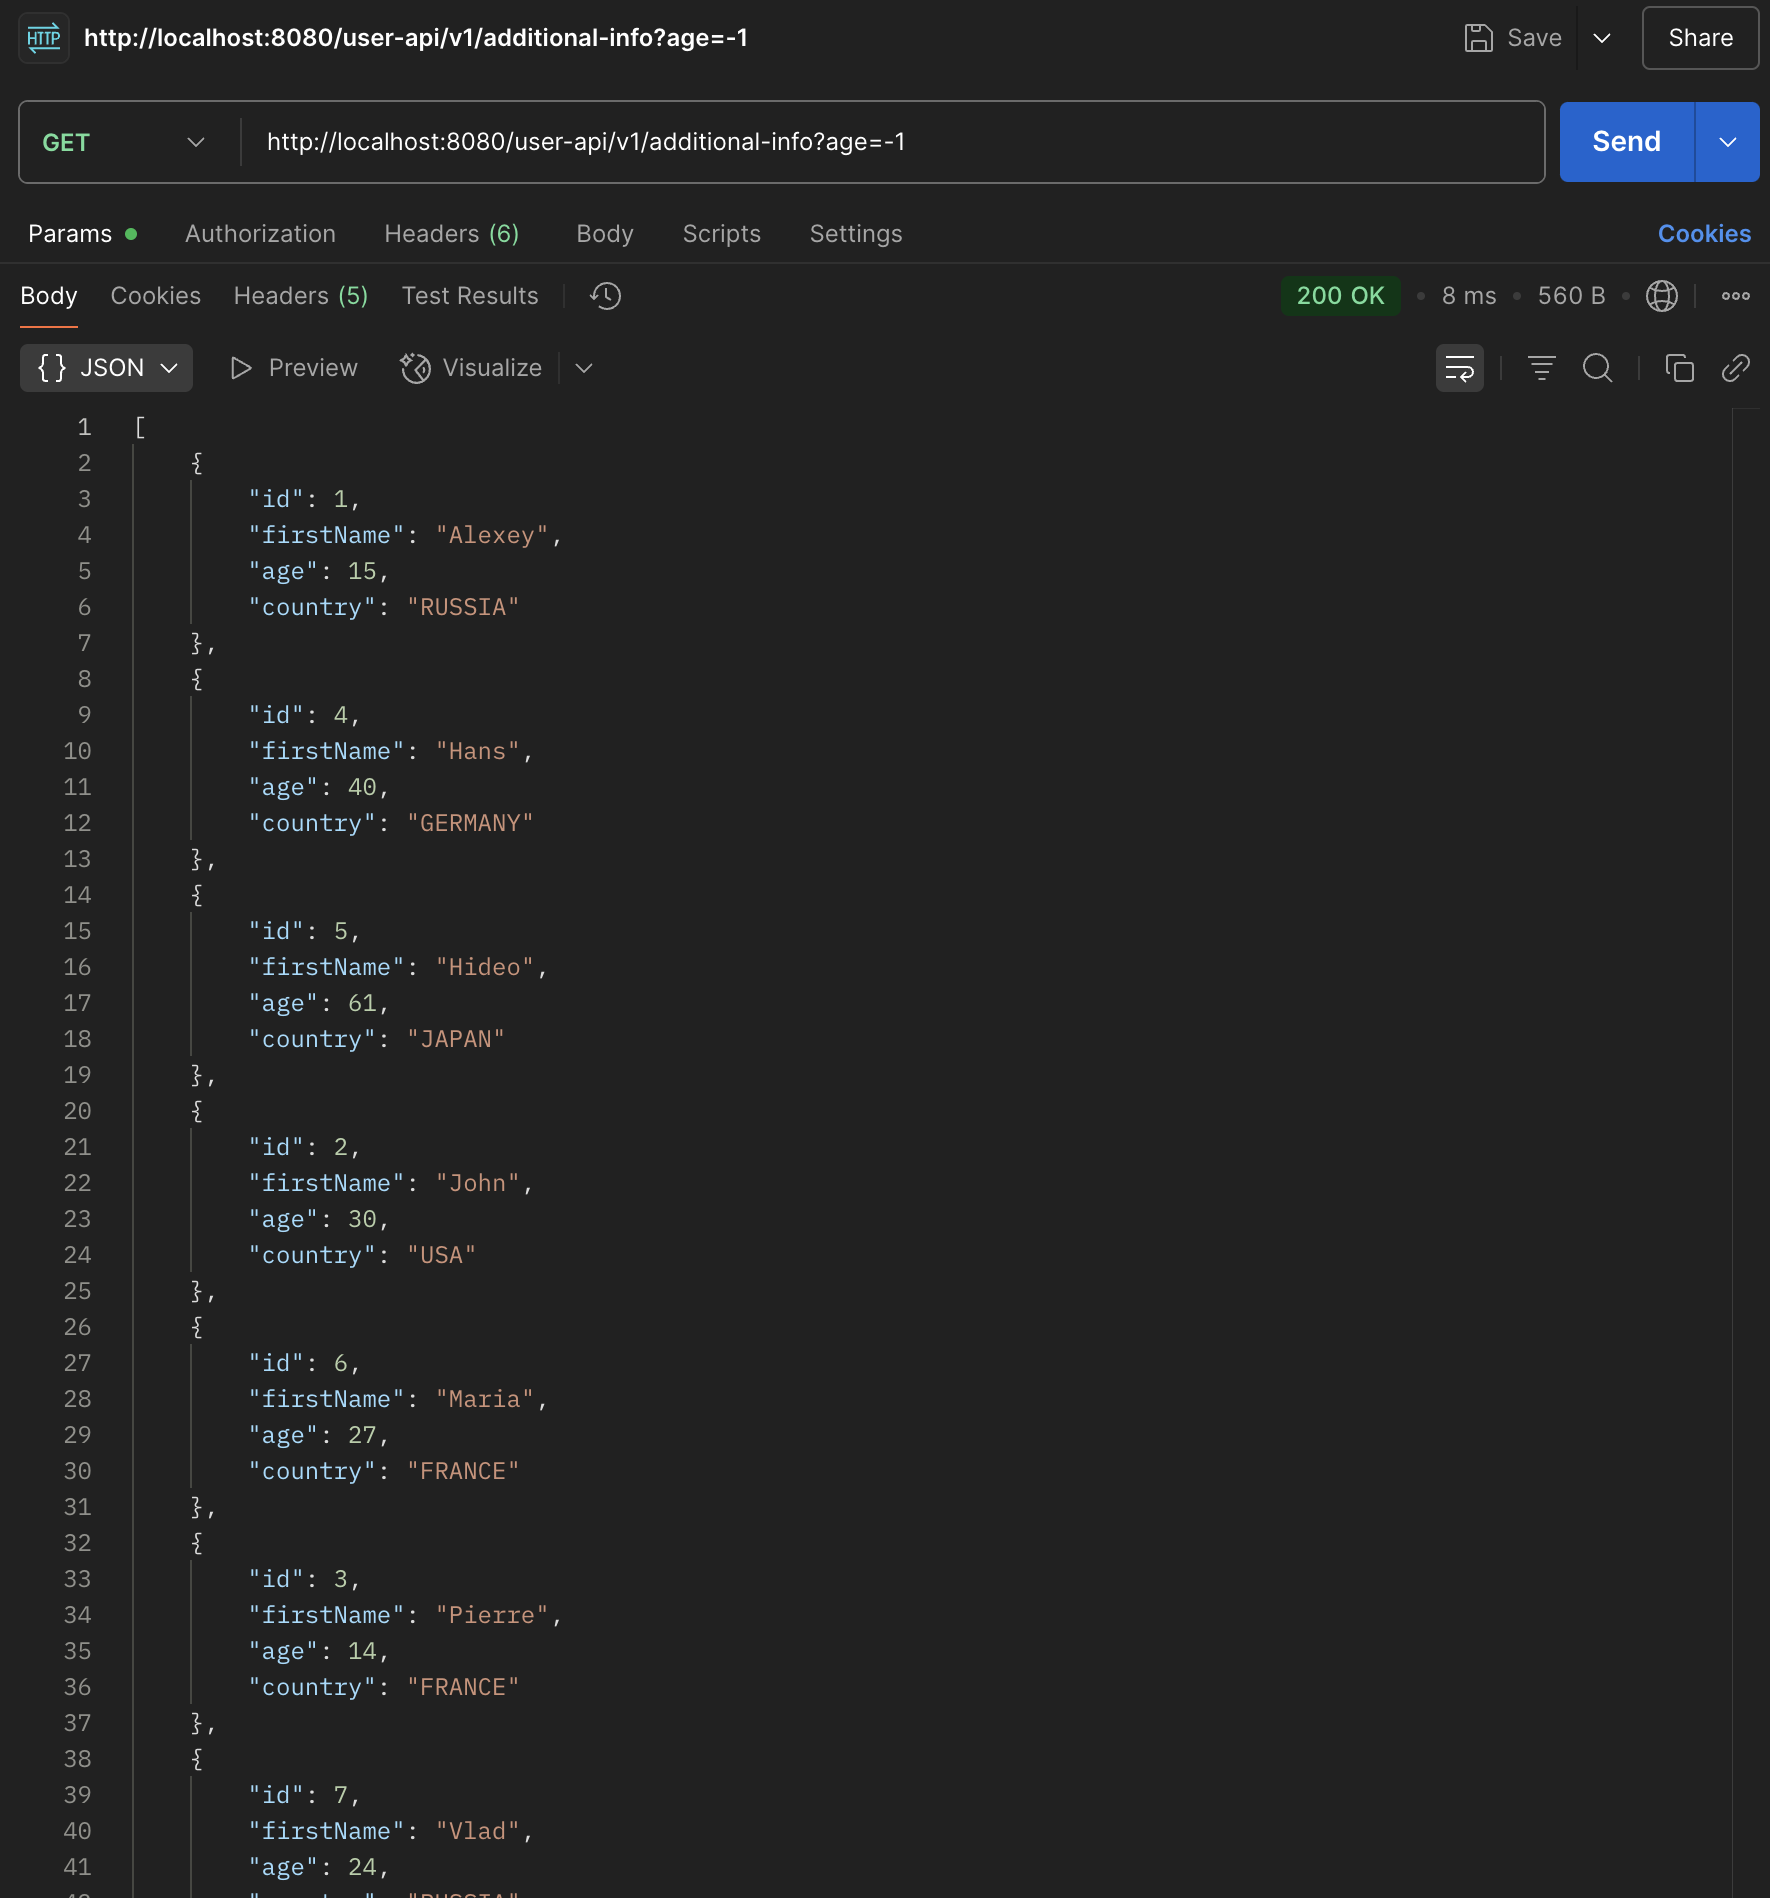
\includegraphics[width=15cm]{resources/11.png}
	\caption{Отрицательное число в age}
\end{figure}

Нам вернутся все пользователи, но отсортированные по имени по алфавиту.

Запишем в age 30:

\begin{figure}[H]
	\centering
	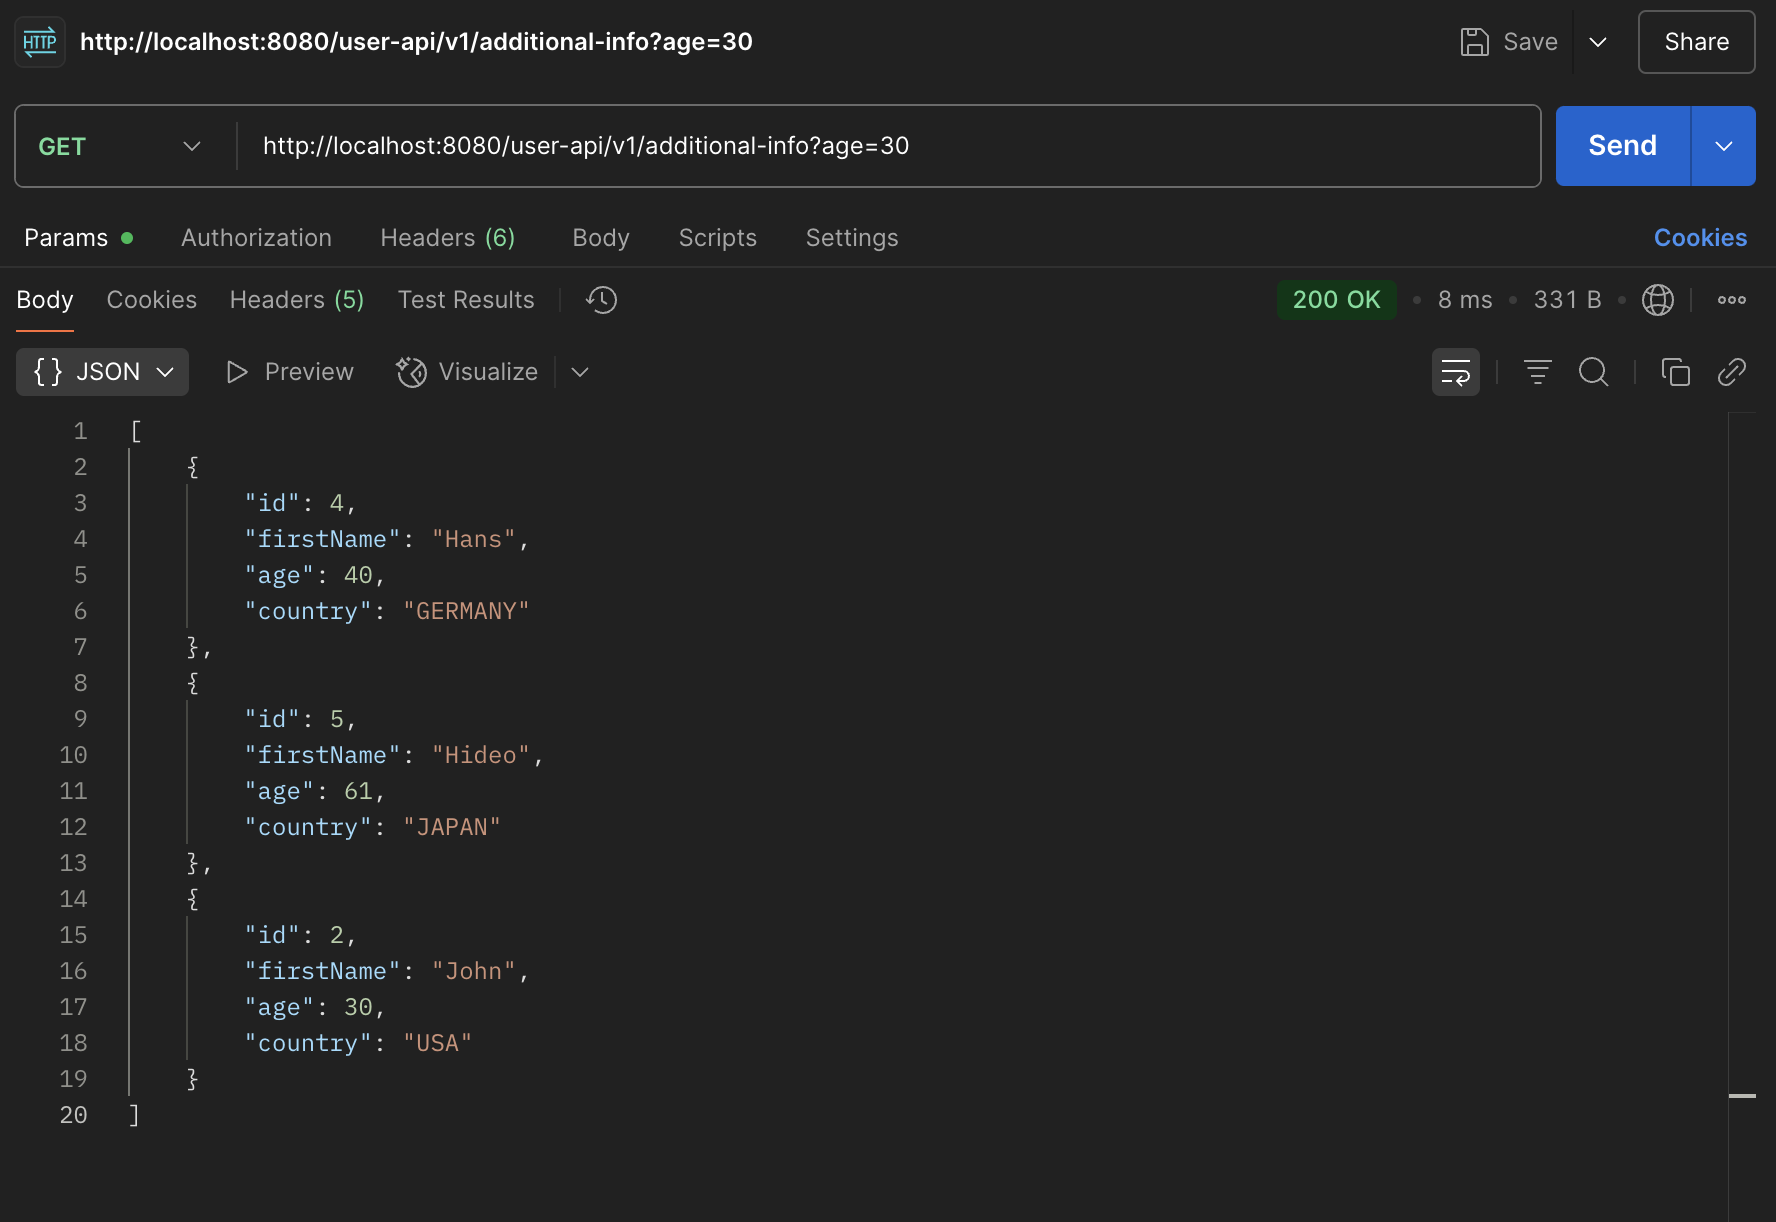
\includegraphics[width=15cm]{resources/12.png}
	\caption{Число 30 в age}
\end{figure}

Нам вернутся только пользователи с возрастом 30 и выше, отсортированные по имени по алфавиту.

Наконец, запишем в age 80:

\begin{figure}[H]
	\centering
	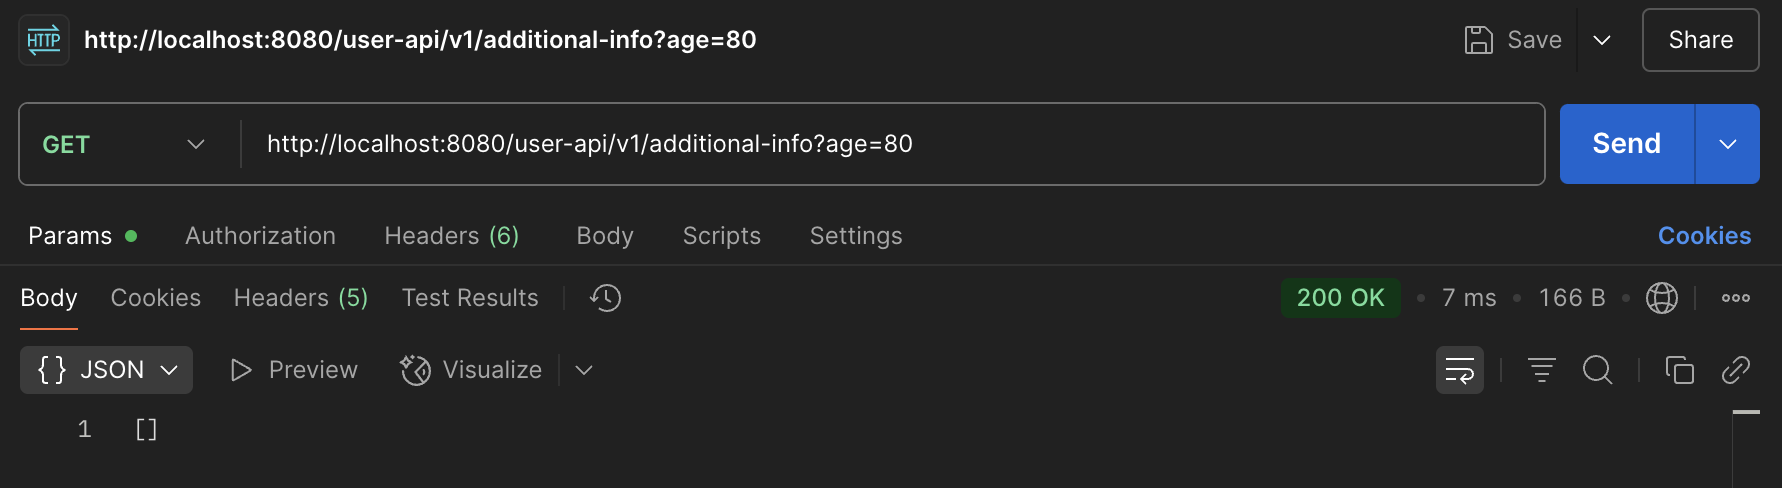
\includegraphics[width=15cm]{resources/13.png}
	\caption{Число 80 в age}
\end{figure}

И закономерно получим пустой список пользователей.

Для верности заглянем в базу данных через админ-панель:

\begin{figure}[H]
	\centering
	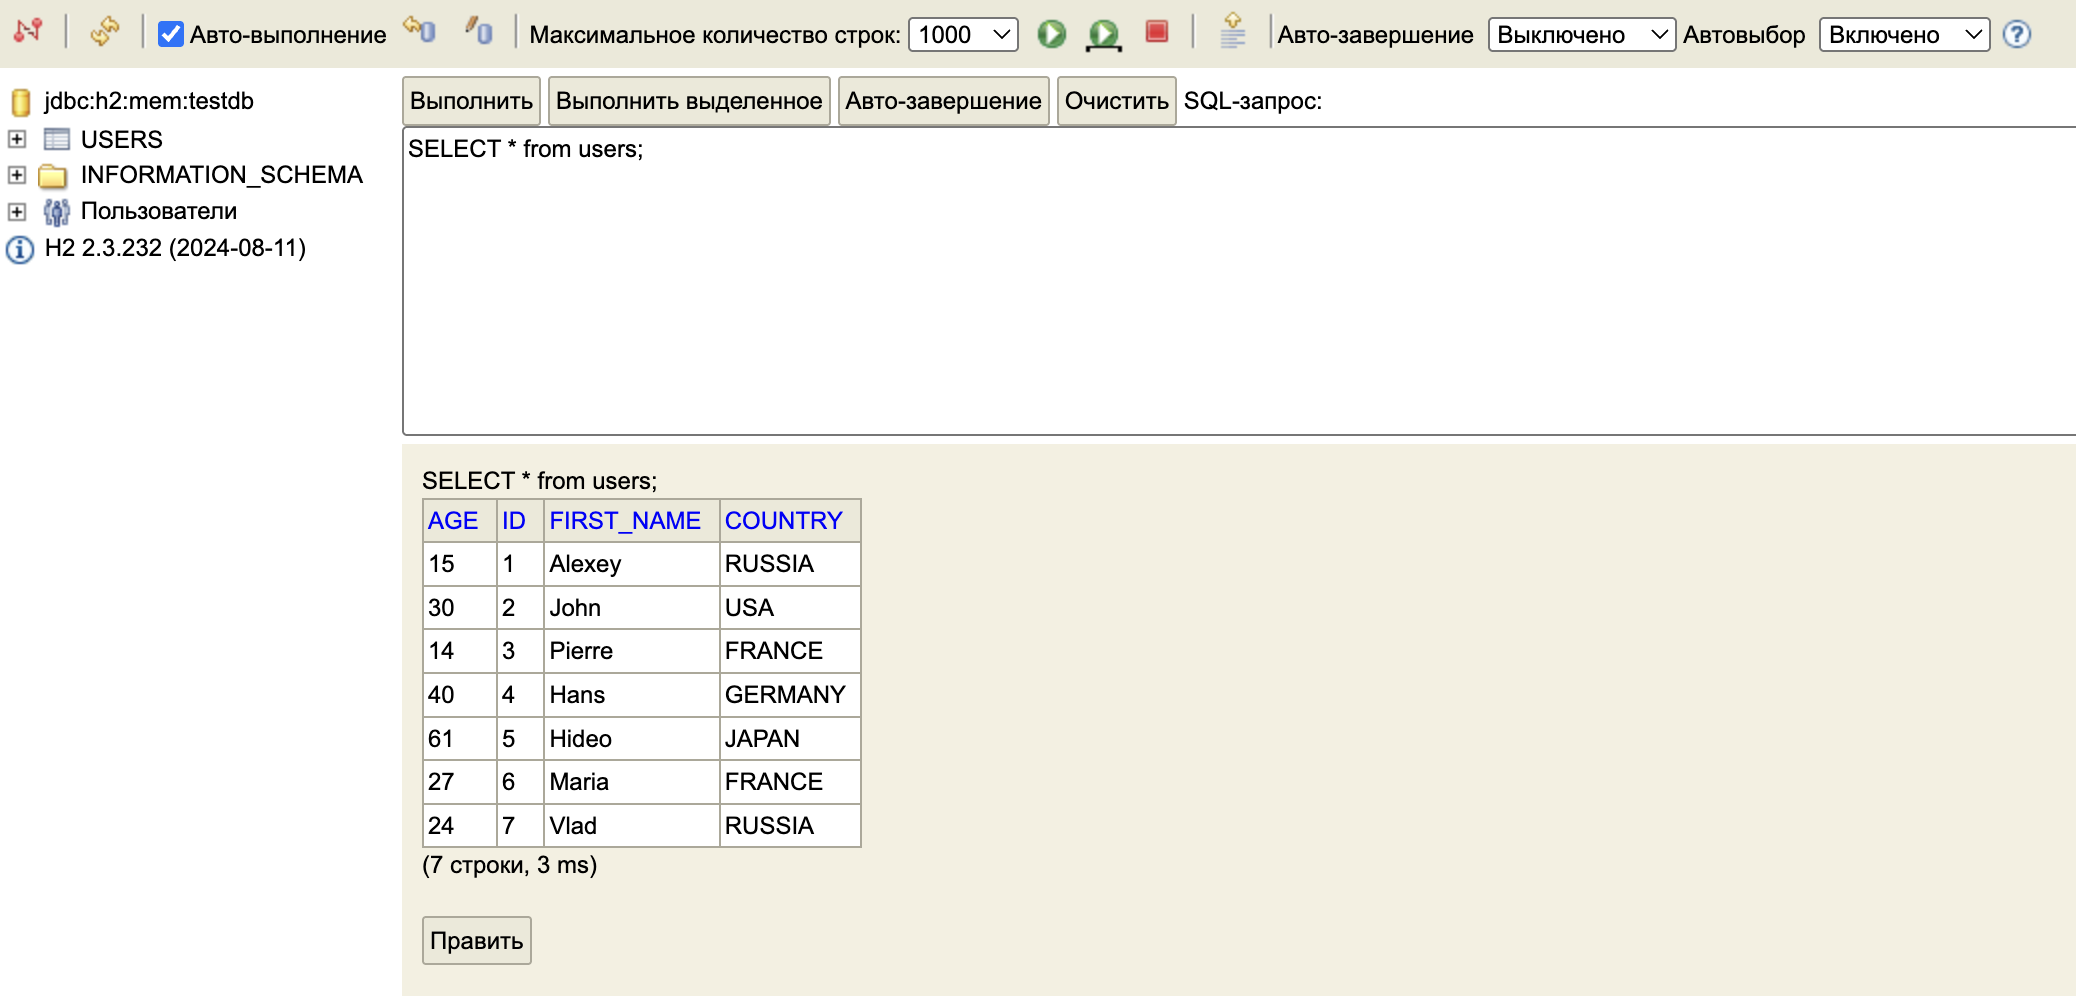
\includegraphics[width=15cm]{resources/14.png}
	\caption{Админ-панель после добавления пользователей}
\end{figure}

Увидим, что добавленные нами пользователи также там появились.

Также интересно посмотреть, что происходило в консоли во время наших запросов:

\begin{figure}[H]
	\centering
	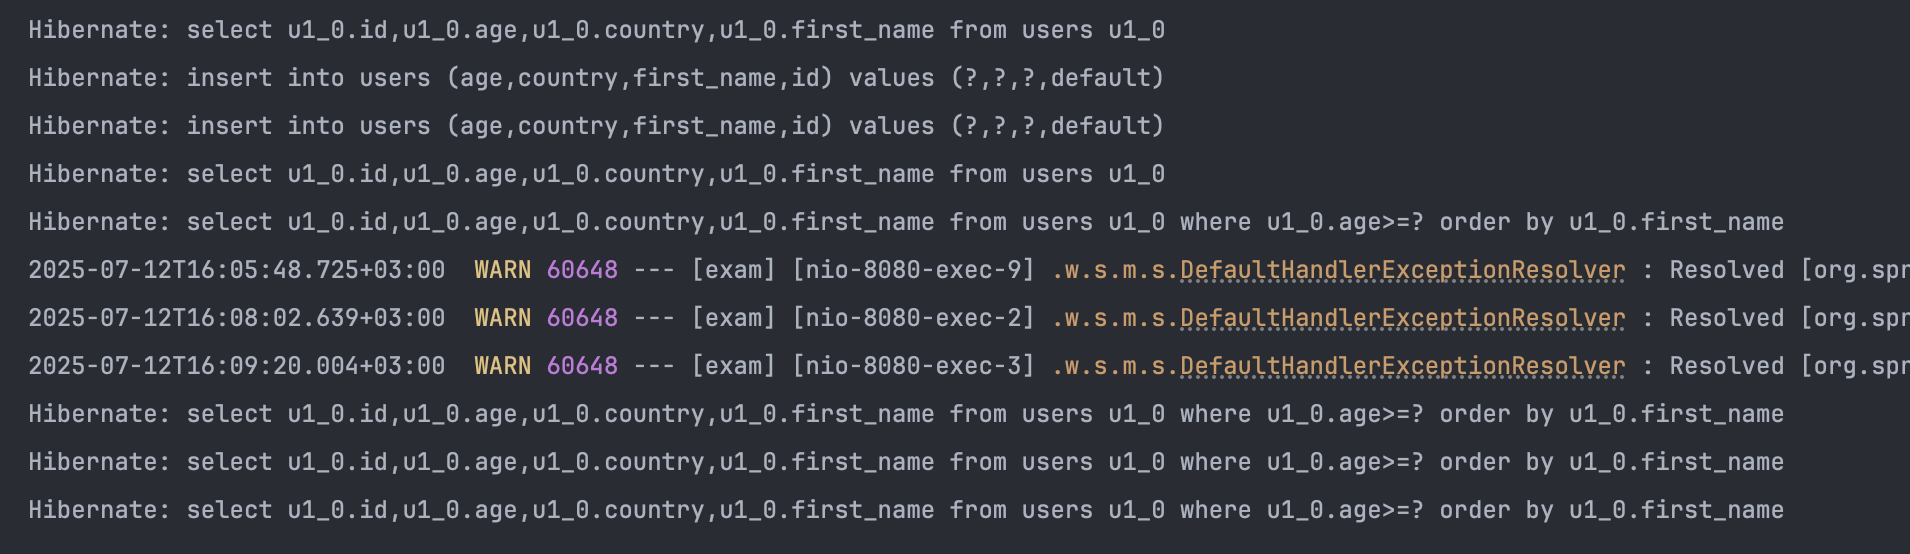
\includegraphics[width=15cm]{resources/15.png}
	\caption{Консоль во время запросов}
\end{figure}

Hibernate переводил наш код в обычные SQL запросы и выполнял их, а когда мы вводили некорректные данные для age - срабатывал \texttt{DefaultHandlerExceptionResolver} (он вызывается 3 раза, а не два, поскольку я вызвал метод с некорректным age еще один лишний раз).

\newpage
\section{Заключение}

В ходе выполнения задания было разработано и протестировано простое Spring Boot веб-приложение, реализующее работу с сущностью пользователя в in-memory базе данных H2.

Все требования технического задания были выполнены: реализованы необходимые REST-эндпоинты, соблюдена многослойная архитектура, обеспечена пользователей при старте.

Работа позволила мне повторить навыки проектирования структурированного Java-приложения на Spring Boot, поработать с JPA и настройкой in-memory базы данных, а также отработать основные принципы построения REST API. Применяя данные принципы можно расширять данное приложение, а также создавать новые.

\end{document}